\documentclass[officiallayout]{tktla}
%\documentclass[officiallayout,a4frame]{tktla}
\usepackage[utf8]{inputenc}
\usepackage{latexsym}
\usepackage{graphicx}
\usepackage[
  backend=biber,
  bibstyle=ieee,
  citestyle=numeric-comp,
    sortlocale=en_US,
    natbib=true,
    url=false, 
    doi=true,
    eprint=false
]{biblatex}
\usepackage{software-biblatex}
\usepackage{pdfpages}
\usepackage[hidelinks]{hyperref}

% Math environments and symbols
\usepackage{amsmath}
\usepackage{amsfonts}

% Lemma environment
%\newtheorem{theorem}{Theorem}[section]
%\newtheorem{lemma}[theorem]{Lemma}

% Independence symbol
\newcommand\indept{\protect\mathpalette{\protect\independenT}{\perp}}
\def\independenT#1#2{\mathrel{\rlap{$#1#2$}\mkern2mu{#1#2}}}

% For thesis papers section
\usepackage{geometry}
\def \dvWHITE{white}
\def \dvBLACK{black}
\def \dvBLUE{blue}
\def \dvGREEN{green}
\def \dvheight{231pt}
% Creates black box with the text given as first parameter in white
\newcommand\note[3] {\marginpar{\vspace{#2}\colorbox{#3}{\parbox[c][\dvheight][t]{34.8pt}{\vspace{0.3cm}\color{white}\centering\Huge{\textbf{#1}}}}}}

% Footnotes without numbering
\let\svthefootnote\thefootnote

\addbibresource{maklin2022.bib}

\title{Probabilistic methods for \\ high-resolution metagenomics}
\author{Tommi Mäklin}
\authorcontact{tommi@maklin.fi\par
  https://maklin.fi/}
\pubtime{June}{2022}
\reportno{0}
\isbnpaperback{000-00-0000-0}
\isbnpdf{000-00-0000-0}
\issn{1238-8645}
\issnonline{2814-4031}
\printhouse{Unigrafia}
\pubpages{7} % --- remember to update this! 
% For monographs, the number of the last page of the list of references
% For article-based theses, the number of the last page of the list of
% references of the preamble part + the total number of the pages of
% the original articles and interleaf pages.
\supervisorlist{Antti Honkela, University of Helsinki, Finland \\ \hspace{8pt} Jukka Corander, University of Oslo, Norway}
\preexaminera{Exam Iner, University of Examinations, Exaministan}
\preexaminerb{Read Er, University of Examinations, Exaministan}
\opponent{Oppo Nent, University of Endless Argumentation, The Argumentlands}
\custos{Antti Honkela, University of Helsinki, Finland}
\generalterms{Algorithms, Experimentation}
\additionalkeywords{genomic epidemiology, plate sweeps, probabilistic modeling, pathogen surveillance, taxonomic profiling, taxonomic binning, metagenomics}
% Computing Reviews 1998 style
%\crcshort{A.0, C.0.0}
%\crclong{
%\item[A.0] Example Category
%\item[C.0.0] Another Example
%}
% Computing Reviews 2012 style
\crclong{
\item Mathematics of computing $\rightarrow$ Probability and statistics $\rightarrow$ Statistical computing
\item Computing applications $\rightarrow$ Biosciences
}

\permissionnotice{
  Doctoral dissertation, to be presented for public examination with 
  the permission of the Faculty of Science of the University of
  Helsinki in \ldots{} on \ldots{} at XX o'clock. Fill in the examination
  venue, date and time into the previous sentence.
}

\newtheorem{theorem}{Theorem}[chapter]
\newenvironment{proof}{\noindent\textbf{Proof.} }{$\Box$}

\begin{document}

\frontmatter

\maketitle

\begin{abstract}
  rewrite \citet{maklin_high-resolution_2021} a \citep{maklin_bacterial_2021}

\end{abstract}

\begin{acknowledgements}
  Olvi (III) \\ \& Koff IVA
   \begin{flushright}
  Rv  rip, June 2022\\
  Tommi Mäklin
  \end{flushright}
\end{acknowledgements}

\tableofcontents

\mainmatter

\chapter{Introduction}

In the past decades research focusing on bacterial pathogens has
largely been driven by analysis of the contents of bacterial genomes
obtained by whole-genome sequencing. Although the price of sequencing
itself has decreased tremendously during this timeframe, most analyses
still rely on using sequence data from pure bacterial cultures created
by isolating a bacterium from an initial mixed culture. Since these
cultures are created by cultivating environmental samples, they
typically contain several distinct bacteria \textemdash and other
microorganisms \textemdash that a thorough analysis would aim to
isolate in a pure culture. In practice, the number of isolations that
can be performed is limited and preparing large numbers of samples for
DNA sequencing rapidly becomes a significant economical barrier even
in well-resourced public health laboratories.

The typical use for sequencing data in public health settings is
genomic epidemiology, where researchers are interested analysing the
genomes of the pathogens to trace their transmission and spread. For
example, comparing mutations in the genomes of a pathogen isolated
from several patients during an epidemic may aid in inferring the
transmission chain by elucidating the short-term evolutionary
history. Similarly the long-term history can be inferred by looking
for larger structural changes, horizontal gene transfer, and
accumulated mutations in genomes assembled from the sequence data. If
the sequencing is performed routinely and the data is made publicly
available, the reporting from several laboratories may be combined to
create an extremely valuable resource for both researchers and
policymakers. However, the vast majority of genomic epidemiological
analyses require high coverage and high quality sequence data to
achieve meaningful resolution, which has translated to dominance of
the expensive pure-colony isolation approach in data generation.

Recently, shotgun metagenomics, where DNA is extracted and sequenced
directly from the original environmental sample, has emerged as a
potential cost-effective alternative to pure whole-genome
sequencing. Although this approach conveniently gets around both the
economic barrier and potential biases introduced by the cultivation
steps, direct sequencing often requires significantly higher
sequencing depths. Sequencing at depths typical to isolate analyses
often results in excess amounts of host DNA and fails to provide
sufficient resolution for the more elusive members of the microbiome
that are present only at low abundances. Due to these factors, shotgun
metagenomics may be difficult to apply in situations where researchers
are only interested in some subset of bacteria but wish to perform
analyses that require high sequencing depth.

When choosing between shotgun metagenomics and isolate sequencing, a
middle-ground can be found in creating the initial mixed culture but
skipping the isolation steps and instead sweeping and sequencing the
mixed culture. Since culture media are available for most clinically
relevant bacteria, this approach allows enrichment of the species of
interest while simultaneously filtering out host DNA, effectively
avoiding the pitfalls in both isolate and shotgun metagenomics by
limiting the diversity of the sample. Accordingly, this approach is
sometimes called limited-diversity metagenomics
\citep{cocker_drivers_2022} but will be referred to as plate sweep
metagenomics in this thesis.

Although both plate sweep metagenomics and shotgun metagenomics
have technically been possible for many years, the development of
computational methods has largely focused on analysing data from pure
cultures. Although some advances have been made in developing
computational tools capable of identifying the taxonomic composition
of a set of reads (taxonomic profiling) or assigning the individual
sequencing reads to their taxonomic origins (taxonomic binning), the
accuracy of these tools is significantly hindered in the presence of
within-species variation. In practice such variation is ubiquitous in
both clinical and envinronmental samples, rendering many of the tools
difficult to use when within-species level information is required.

In this thesis I present research that enables both taxonomic
profiling and binning from either metagenomic or plate sweep
sequencing data using computational methods. While the methods were
initially developed for plate sweeps metagenomics work, I also
demonstrate that they can reliably be applied to whole metagenome
sequencing data as well. Using either of the two approaches to
generate metagenomic sequencing data enables performing completely new
types of analyses which are also briefly covered.

The first two articles included in this thesis contain descriptions of
the aforementioned two methods. The first of these methods, called
mSWEEP, provides a probabilistic model for taxonomic profiling of
bacteria at within-species lineage level based on pseudoalignments
against a set of reference sequences. The second method, mGEMS,
leverages the information from mSWEEP to construct an assignment rule
for taxonomic binning of sequencing reads to bins that correspond to
the lineages. Both methods rely on the fundamentally important insight
that each sequencing read can - and should - pseudoalign and be
assigned to several lineages within the species at once. By combining
the two methods, sequencing data from samples containing several
lineages of the same species can be computationally demixed and used
to obtain results that are nearly indistinguishable from the results
of using isolate data.

While the methods from the first two articles are designed with direct
analysis of sequencing data from mixed cultures in mind, the third
article shows that both methods are applicable even when the initial
plating step is skipped and the sequencing data is derived directly
from an environmental sample. Thus, in the third article I have
analysed such samples from babies born in the UK collected during
their neonatal period and discovered several results showing strong
competition between bacterial species and strains during the initial
colonization of the gut microbiome. More importantly, from a methods
perspective, this analysis shows that mSWEEP and mGEMS provide
(so-far) completely unprecedented levels of resolution in analysis of
metagenomic sequencing data.

Together the three articles in this thesis represent foundational
methodological steps in both opening up high-resolution exploration of
bacterial diversity as well as making such analyses more accessible to
resource-constrained laboratories.

\section{Three approaches to sequencing bacterial DNA}
\label{three-approaches-to-metagenomics}

%- Something about sequeuncing reads and sequence assembly? 16S sequencing?

Preparing bacterial DNA for sequeuncing is typically done after a
culture step, where a sample is streaked across a culture plate or
immersed in liquid and then inoculated for some amount of time to
allow the bacteria to multiply and grow on the culture
plate. Alternatively, in metagenomics sequencing the culture step is
skipped and DNA is extracted directly from the sample along with the
DNA from any other organisms that may be present. When it comes to the
end-result, the sequencing reads, both approaches have their
advantages and disadvantages, which are covered in more detail in this
section.

Metagenomics sequencing, where all DNA in a sample is extracted
(Figure \ref{fig:microbiome-sampling-methods}a), has emerged as a tool
to analyse the full breadth of the microbiome. Metagenomics
conveniently avoids the biases introduced by approaches that include a
culture step and has consequently revealed an enormous diversity of
bacterial species that are not able to grow or compete on commonly
used culture media. However, exploring this diversity comes at a price
since the produced sequencing reads are split across the numerous
bacteria present, resulting in a prohibitively high sequencing depth
requirement for analysis of the less abundant taxa. This has rendered
the metagenomic approach difficult to apply in for example clinical
research, where the interesting bacteria (pathogens) are often only a
small part of the microbiome but the typical analyses require large
numbers of reads to produce accurate results.

Incorporating a culture step on a medium that selects for the bacteria
interest provides means to avoid wasting sequencing efforts on
uninteresting taxa. This approach allows for generating large numbers
of sequencing reads from the bacteria that grow to dominate the
culture, which in turn enables detailed analyses such as SNP calling
or identifying antimicrobial resistance genes. When the sequencing is
performed on the plate created from the sample, including all
bacterial species and strains that grow there, the approach is called
plate sweep metagenomics (Figure
\ref{fig:microbiome-sampling-methods}b). Although this approach has
not been previously widely used in the literature due to difficulties
in separating very closely related bacteria, it is a major application
area for the methods presented in this thesis due to the inherent
advantage of focusing sequencing resources on only the relevant
bacteria.

\noindent\let\thefootnote\relax\footnote{Figure source: Adapted from \cite{praveera_fenugreek-sprouts} and \cite{niaid_escherichia-coli}. Released under the \href{https://creativecommons.org/licenses/by-sa/4.0}{CC BY-SA 4.0 license}.}
\addtocounter{footnote}{-1}\let\thefootnote\svthefootnote
\begin{figure}[!ht]
  \label{fig:microbiome-sampling-methods}
    \centering
    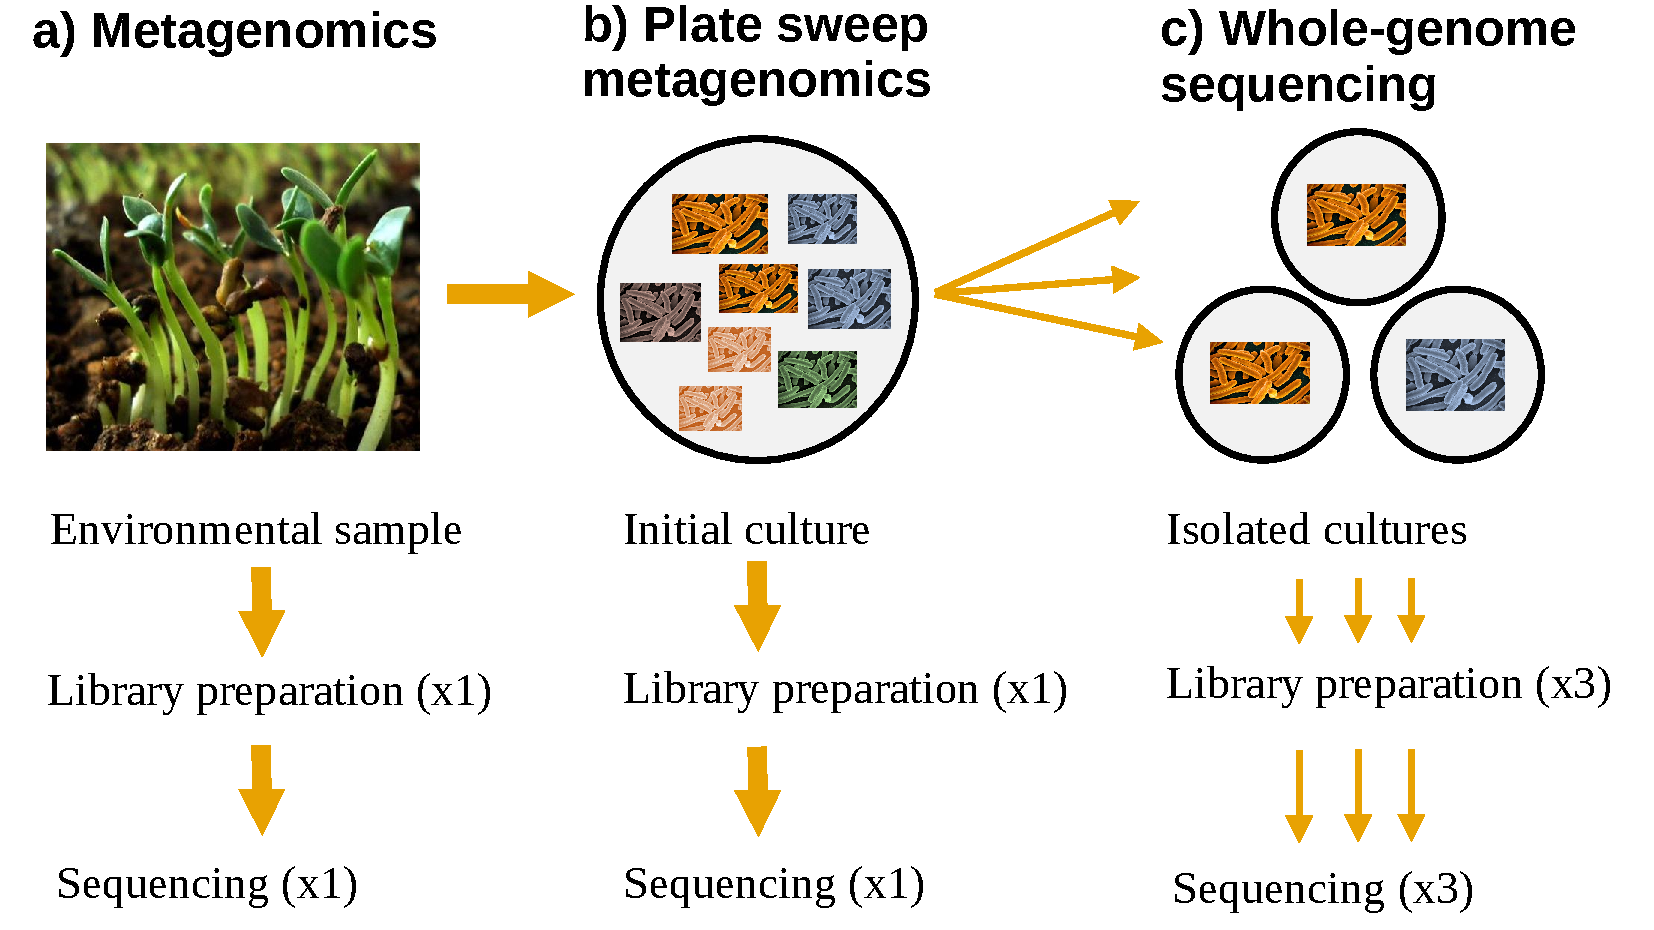
\includegraphics[width=\textwidth,keepaspectratio]{img/sampling/microbiome_sampling_methods.pdf}
    \caption{Different approaches to sequencing bacterial DNA. Panel \textbf{a)} depicts the metagenomic approach, where sequence data is collected directly from the environmental sample. Panel \textbf{b)} depicts the plate sweep metagenomic approach, where the environmental sample is plated on a selective medium and DNA is sequenced from the whole plate. Panel \textbf{c)} depicts the whole-genome sequencing approach, where a subset of visible colonies on the selective medium are picked, cultured again on their own plates, and then sequenced. The orange arrows depict steps that require laboratory work.}
\end{figure}

The third approach leverages a second culture step, where visible
colonies are picked from the initial culture and transferred to their
own culture plates. After letting the new plates inoculate, the
resulting culture will (presumably) contain only clones of the
bacteria that formed the colony that was picked. Since this approach
gets rid of all of the variation in both the sample and the initial
culture, resulting in massive numbers of sequencing reads from the
same genome, it is accordingly called whole-genome sequencing (Figure
\ref{fig:microbiome-sampling-methods}c). While this approach allows
accurate recovery of the genome of a single bacterial strain, the
number of colony picks that can be performed is often limited and some
sort of heuristic is required to select which colonies to pick.

In epidemiological analyses, the whole-genome sequencing approach has
so-far dominated the field due to its ability to produce highly
accurate data. However, transitioning sequencing efforts to either
metagenomics or plate sweep metagenomics has obvious benefits in both
upscaling the amount of samples that can be processed and in providing
better representation for both species and strain-level diversity in
the samples. Unfortunately the accuracy from existing tools has not
been as good as required but with recent developments in sequence
assembly and/or taxonomic binning \& profiling from metagenome-derived
sequencing data, the new frontier may finally be opening for
exploration.

\section{Analysing metagenomic sequence data}

\textbf{- Need a picture of the different approaches.}

Sequencing data from a metagenomic source presents several challenges
to bioinformaticians. Firstly, the increased diversity of species
requires much larger computational resources to analyse. Secondly, the
possible pressence of strain-level variation vastly complicates
analyses that rely on separating the reads to distinct taxonomic units
since the differences between strains of a bacteria can be minimal to
the level of being confused with sequencing error. Subsequently, most
of the methods development has focused on operating at the
species-level with the assumption that only one strain from each
species is present at the same time. In this section I will briefly
cover the previous approaches and introduce the principal differences
between them and mSWEEP and mGEMS.

Metagenome assemblers are one of the more used tools for analysing
metagenomic sequencing data. These assemblers aim to produce
assemblies directly from the sequencing reads, similarly to sequence
assembly in isolate sequencing but taking into account the different
taxons possibly present. Often, the assemblers work under the
assumption that the taxons in the reads are distinct enough that their
assembly graphs do not overlap. While this approach works fine when
the data contains taxons that are separated by long evolutionary
distances, it can fail in the presence of closely related strains of
the same species or even species of the same genus. Nevertheless,
metagenome assemblers have found a great deal of use in settings where
the data is assumed to contain many organisms that are, presumably,
unculturable or have not been encountered before.

Taxonomic profilers and taxonomic binners approach the metagenomics
problem from a slightly more detailed point of view. Taxonomic
profilers attempt to assign (relative) abundances to some sets of
reference data, or reference taxons, found in the reads, and taxonomic
binners attempt to create read bins that correspond to some reference
taxon. These two approaches often go hand-in-hand in that the
taxonomic profiles can be extracted by counting the reads in each bin
but some approaches still exist that attempt only the profiling
task.

Yet another category of metagenomics data analysis can be found in
approaches that do not attempt the previously mentioned tasks but
rather compare different samples to each other. These approaches
typically aim to infer similarity and, through that, transmission
events or shared strains between some samples. While these can be
extremely accurate especially in transmission analysis, these
approaches often cannot distinguish between different strains in the
sample and do not have the capability to perform analyses that require
access to the genomes of the individual strains. However, they can
provide information that would otherwise require analysing a large
number of genomes (in the case of perfect information i. e. a perfect
taxonomic binner) and have found much use in that regard.

Both profiling and binning methods can further be divided into
those that leverage reference data and those that attempt
reference-free estimation. While reference-free estimation can yield
data from previously unknow species or strains, reference-based
approaches typically obtain higher resolution. Leveraging reference
data is one of the central aspects of the work in this thesis to
perform both taxonomic profiling (mSWEEP) and taxonomic binning
(mGEMS), and the benefits of a reference-based approach will be
explored in more detail later on.

These metagenomics approaches have found widespread aplications in
analysing sequencing data from highly complex environments - such as
soil samples. Especially the reference-free approaches have proved
highly useful in cases where the contents of a sample bear little
similarity to previously sequenced samples. However, these scenarios
are becoming increasingly scarce with more widespread availability of
sequence data and new culture methods developed for species previously
thought unculturable. Especialy in clinical settings, where the
bacterial diversity is rather well known and has been studied for many
years, it is uncommon to come across an entirely new (pathogenic)
species. In these cases, adding information in the form of reference
sequences typically results in much higher ceiling for the possible
resolution.

In the class of metagenomics analyses, the approach presented in this
thesis falls broadly in reference-baesd taxonomic profiler and
taxonomic binner category. However, our approach differs from previous
research in that rather than trying to assign relative abundances to a
set of reference sequences, we attempt to assign abundances to a
reference \textit{lineage} - i. e. some group of reference sequences
that is somehow related to each other. This approach has the benefit
of covering the possible variation in a reference lineage, which
typically present problems for reference-based metagenomics
tools. Additionally, our tool works with bespoke sets of reference
sequences, which means that it can be applied to explore the diversity
of a specific species in great detail while excluding the
uninteresting species. While this discards some data that might be
useful, the approach greatly simplifies the modelling task, allowing
for a much higher accuracy in the exploration of within-species
variation.

\section{Genomic epidemiology as a tool for pathogen surveillance}

\textbf{Figure about genomic epidemiology analyses}

The other significant aspect of this thesis has to do with tracing the
spread of pathogens using sequence data, called genomic
epidemiology. In recent years, the use of genome-informed analyses has
greatly expanded the capability of researchers to track and trace
pathogens and identify genetic elements relevant for e. g. antibiotics
resistance and pathogenesis. This analysis has typically been
performed using isolate sequencing data, which provides great detail
into a single bacterial genome but has some downsides covered in the
previous sections. One important goal of the thesis work has been to
provide tools that extend the analysis capabilities to metagenomic
data from either plate sweeps or whole-genome shotgun sequencing.

Combining the genomic sequences of pathogens with data about the time,
location, and other clinically relevant features provides clinical
practitioners, policy makers, and researchers with a much wider
perspective into transmission and evolutionary analysis than using
either of the information alone. This has enabled several significant
advantages in e.g. analysis of the transmission of plasmids and
targeting vaccine design, as well as in providing novel insights into
several causative agents of disease that could not be identified
without including genome information. With the price of sequencing
constantly decreasing, genomics-driven analysis has high potential to
further revolutionize the way we think about disease.

Incorporating metagenomics data into genomic epidemiological analyses
presents the next obvious frontier. Since the microbiome is in
practice nearly universally composed of several interacting
micro-organisms, there is a high possibility that excluding some parts
may miss otherwise relevant information. For example, in a recent
study (Gerry's), the pathogen \textit{S. pneumonimae} was found to
often co-colonize patients with a dominant strain and a nondominant
strain. In the developed world, vaccine development has targeted the
dominant strain but entirely ignored the nondominant strain, which has
not been identified with previous methods. The nondominant strain
does, however, have the capability to cause the same disease and is,
in fact, the leading cause in the developing world. The results from
this study highlight that by focusing only on the non-metagenomic
contents of the microbiome, potentially significant information is
missed.

Another aspect in favour of using a more metagenomics-oriented
approach arises from simple practicality: sequencing several taxons at
once is simply more cost-effective than performing many isolations, as
covered in the previous sections. Using a metagenomics-oriented
approach makes the analyses much more widely available in the form of
significant cost reductions. This means that analyses which would not
be possible to perform in locations lacking funding and resources
might find a way through the use of metagenomic sequencing. Currently
especially data from lower-middle income countries is scarce due to
the limited sequencing capability which metagenomics has the potential
address. Furthermore, performing metagenomics sequencing alongside the
traditional sequencing types has the potential to preserve data from
the samples for future analyses, should methods capable for more
detailed exploration become available.

In conclusion, the already relatively recent field of genomic
epidemiology can be seen as underogoing a transform into becoming
widespread public practice. With the development of methods - such as
the ones presented in this thesis - capable of lowering the costs and
increasing the resolution, the field will likely produce significant
discoveries through the inclusion of metagenomics data.

\section{Contributions}

This thesis comprises three publications covering both mSWEEP and
mGEMS as well as a third article demonstrating their application to
whole-genome shotgun metagenomic sequencing data. The first two
publications are accompanied by software implementations. The third
article is more applied in nature, exploring in more detail the types
of analyses enabled by the first two papers.

\subsection*{Paper I \textemdash High-resolution sweep metagenomics using fast probabilistic inference}
By \underline{Tommi Mäklin}, Teemu Kallonen, Sophia David, Christine J
Boinett, Ben Pascoe, Guillaume Méric, David M Aanensen, Edward J Feil,
Stephen Baker, Julian Parkhill, Samuel K Sheppard, Jukka Corander, and
Antti Honkela. Published in \textit{Wellcome Open Research} (2021),
5:14, doi: 10.12688/wellcomeopenres.15639.2.

In the first paper, we presented and benchmarked the mSWEEP method for
taxonomic profiling of sequencing data containing multiple strains
from the same bacterial species. My contributions included development
and implementation of the method, designing the benchmarks and
comparisons with similar methods, running all analyses with mSWEEP,
writing the manuscript, and to reviewing and editing the article.

Software implementation of the ideas presented in Paper I is
available from GitHub at
\href{https://github.com/PROBIC/mSWEEP}{PROBIC/mSWEEP} (latest
version). The latest version at the time of writing is archived and
available in Zenodo \citep{maklin_mSWEEP}.

\subsection*{Paper II \textemdash Bacterial genomic epidemiology with mixed samples}
By \underline{Tommi Mäklin}, Teemu Kallonen, Jarno Alanko, Ørjan
Samuelsen, Kristin Hegstad, Veli Mäkinen, Jukka Corander, Eva Heinz,
and Antti Honkela. Published in \textit{Microbial Genomics} (2021)
7.11, doi: 10.1099/mgen.0.000691.

The second paper continued to build upon mSWEEP by developing an
algorithm for taxonomic binning at within-species variation level,
called mGEMS. I contributed to the development of both the mGEMS
binning algorithm and the full mGEMS pipeline, designing the synthetic
and the \textit{in vitro} benchmark experiments, running the analyses
and creating the visualisations, interpreting the results and writing
the article, and to reviewing and editing the article.

Software implementation of the ideas presented in Paper II is
available from GitHub at
\href{https://github.com/PROBIC/mGEMS}{PROBIC/mGEMS} (latest version).
The latest version at the time of writing is archived and available in
Zenodo \citep{maklin_mSWEEP}.

\subsection*{Paper III \textemdash Strong pathogen competition in neonatal gut colonization}
By \underline{Tommi Mäklin}, Harry Thorpe, Anna Pöntinen, Rebecca
Gladstone, Alan McNally, Ørjan Samuelsen, Pål Johnsen, Trevor Lawley,
Antti Honkela, and Jukka Corander. Awaiting peer-review; available
from \textit{bioRxiv} (2022), doi: XXX.XX/XXX.XXX.XXX.

The third paper provides an example of applying mSWEEP and mGEMS to
whole-genome shotgun metagenomics sequencing data and explores the
dynamics of pathogen competition and colonization in the gut
microbiome of babies in their first three weeks of life. My
contributions to this paper include running the mSWEEP/mGEMS pipeline
on all data used in the paper, updating the reference databases for
the investigated species, performing the analysis of the mSWEEP/mGEMS
results for the samples containing \textit{E. coli}, and aiding the
coauthors in analysing the other species. I additionally contributed
to creating the visualisations, interpreting the results, and
naturally to writing the article.

\section{Structure}

The rest of the thesis is structured into three chapters that describe
how the included papers contribute to the topics presented in the
introduction chapter. The first of the three chapters describes the
basic ideas behind the mSWEEP and mGEMS methods and provides
historical context for the parts of the methods that have their
origins within analysis of RNA sequencing data. The second chapter
describes the experimental results from the three papers in more
detail, focusing more on the applied part rather than the theoretical
foundations. The third chapter is more speculative in nature, covering
both the demonstrated epidemiological applications from the papers as
well as exploring potential future avenues for use of the developed
methods. The thesis concludes with a reprinting of the three included
articles.

\chapter{Mixture modeling of sequence data}

- write about Reference data vs Reference-free approach <- might go to intro?

\section{Characteristics of sequence data from bacteria}
\label{section:bacterial-data}

- Write about individual sequence vs cluster based approach.
-- what is a strain? ie how to distinguish between them if we have no reference data

Something about bacterial pathogens are hard to classify taxonomically
and have weird genomes with weird plasmids and stuff.  Lineages are
much much nicer to work with

\section{Sequence alignment}
\label{section:sequence-alignment}
- Significance of alignment in the analyses (themisto vs traditional alignmnt? Could make a small example here in the high-resolution metagenomics section

- Significance of reference databases.

- Building bespoke databases vs. using refseq or something else.

\section{A probabilistic model for sequences from mixed sources}
\label{section:model}

- Historical context from RNA sequencing.

\subsection{Mixture model formulation}

Assume that we have some set of sequencing reads $R = \left\{r_{1},
\dots, r_{N}\right\}, N \in \mathbb{N}_{+}$ that are independent of
each other and identically distributed. We can write down a generative
mixture model for these reads by defining latent indicator variables
$I = \left\{I_{1}, \dots, I_{N}\right\}$ that follow some mixing
proportions $\boldsymbol{\theta} = \left(\theta_{1}, \dots,
\theta_{S}\right), S \in \mathbb{N}_{+}, \sum_{s = 1}^{S} \theta_{s} =
1$. Since we assumed independence between the reads $R$, $r_{j}
\indept r_{i}$ for all $i \neq j, 1 \leq i \leq N, 1 \leq j \leq N$, the joint
distribution for this generative model is
\begin{equation}
  \label{model:joint-distribution}
  p\left(R, I, \boldsymbol\theta\right) = \prod_{n = 1}^{N}p\left(r_{n} \middle| I_{n}\right) p\left(I_{n} \middle| \boldsymbol\theta\right)p\left(\boldsymbol\theta\right).
\end{equation}

Now, assume that for each read $r_{n}, 1 \leq n \leq N$ we observe
alignments $r_{n, s}$ against the reference sequences $s = 1, \dots,
S$. The information contained in $r_{n, s}$ may be anything about the
alignment. Now, further assuming independence between the alignments
against different reference sequences $r_{n, i} \indept r_{n, j}$ for
all $i \neq j, 1 \leq i \leq S, 1 \leq j \leq S$, the joint
distribution from Equation \ref{model:joint-distribution} factorizes
into
\begin{equation}
  \label{model:joint-distribution-factorized}
  p\left(R, I, \boldsymbol\theta\right) = p\left(\boldsymbol\theta\right)\prod_{n = 1}^{N} \prod_{s = 1}^{S} p\left(r_{n, s} \middle| I_{n} = s\right) p\left(I_{n} = s \middle| \boldsymbol\theta\right).
\end{equation}

The model in Equation \ref{model:joint-distribution-factorized}
corresponds to the mixture model that has been historically used in
many contexts, including the predecessor of mSWEEP. Note that in this
model each reference sequence represents a single taxonomic unit, and
the inferred relative abundances $\boldsymbol\theta$ are the
proportions of the same reference sequences.

\subsection{Incorporating grouped reference sequences}

Although the model in Equation
\ref{model:joint-distribution-factorized} performs admirably when the
reference sequences are sufficiently different from each other,
attempts to estimate the relative abundances of individual reference
sequences fail when the degree of relatedness is increased. Especially
when applying the model to reference data containing sequences from
strains of the same bacterial species, the abundances
$\boldsymbol\theta$ tend to become scattered among the most closely
related sequences - even if the correct sequence is contained in the
reference.

To solve this, the model used in BIB incorporated a clustering for the
reference sequences \textemdash meaning that instead of estimating the
reltaive abundancecs $\boldsymbol\theta$ for the individual reference
sequences, the abundance is estimated for the entire cluster. Although
this approach introduces an obvious loss of resolution when compared
to the sequence-based approach, introducing the use of clustering
provides advantages in accomodating for naturally occurring variation
as well as improving the scalability of the inference part by reducing
the number of reference units.

In modelling terms, Equation \ref{model:joint-distribution-factorized}
can be extended by representing alignments against the reference
sequences $r_{n, s}$ via information about alignments against a
representative sequence $r_{n, k}, k = 1, \dots, K, K \ll S$ from the
cluster $k$. With this change, the changes to the model are minimal:
the $s$:s are simply replaced by $k$:s
\begin{equation}
  \label{model:grouped-joint-distribution}
  p\left(R, I, \boldsymbol\theta\right) = p\left(\boldsymbol\theta\right)\prod_{n = 1}^{N} \prod_{k = 1}^{K} p\left(r_{n, k} \middle| I_{n} = k\right) p\left(I_{n} = k \middle| \boldsymbol\theta\right).
\end{equation}
With an appropriate definition of the likelihood term $p\left(r_{n, k}
\middle| I_{n} = k\right)$, this model (the BIB model) corresponds
to the model used by BIB and can solve the inference problem for
several species of bacteria with well-defined clusterings within the
species.

The model of Equation \ref{model:grouped-joint-distribution} has,
however, several issues that render it difficult to apply in some
scenarios. First, the model requires selecting a representative
sequence for each cluster $k$. This selection is by no means an easy
task \textemdash in fact the problem is TODO cite something
.... Secondly, using a representative sequence implies assumptions
about the clustering: namely that there must be minimal variation
within the clusters in terms of genomic contents and that each cluster
is clearly separated from the others. In BIB, the assumptions about
the clustering are solved by using a representative sequence for the
core genome of the cluster. Unfortunately this introduces a third
problem: some bacterial species do not have a stable core genome and
increasing the number of sequences for any species of bacteria tends
to shrink the core genome regardless of its characteristics due to
randomly occurring mutations.

\subsection{Modelling alignments against sequence groups}

mSWEEP solves the issues present in the BIB model by replacing
alignments against representative sequences for the clusters with a
model for alignments against all available reference sequences from
each cluster. Furthermore, since this replacement results in a large
increase in the number of sequences that are aligned against, the
traditional position-based alignment is replaced with
\textit{pseudoalignment} that only returns a $0$ or $1$ indicating
whether the read aligned somewhere within the reference sequence or
not (see Section \ref{section:sequence-alignment} for more
details). Although pseudoalignment reports less information about the
relationship between the reads and the reference sequences than
traditional alignment, the approach is observed to perform excellently
in cases where the BIB model fails and provide similar resolution in
cases where the BIB model performs well.

With the changes in the mSWEEP model, the observations $r_{n, k}$
become the numbers of observed pseudoalignments $r_{n, k}, 0 \leq
r_{n, k} \leq M_{k}$ against the $M_{k}$ sequences assigned to each
cluster $k$. If assumptions about independence between the clusters
are kept, the formulation for the model remains the same as the one
presented in Equation \ref{model:grouped-joint-distribution} with the
only changes being to the likelihood term $p\left(r_{n, k} \middle|
I_{n} = k\right)$.


\subsection{Likelihood for a clustered reference}

When dealing with pseudoalignments against clustered reference
sequences, the likelihood term $p\left(r_{n, k} \middle| I_{n} =
k\right)$ in Equation \ref{model:grouped-joint-distribution} needs to
be carefully defined to account for several factors arising from the
biological facts affecting the structure of the reference. One, the
clusters may vary greatly in size, with some of them having just one
sequence and some of them hundreds or even thousands. Two, due to
sequencing erros, reference errors (assembly errors or lack of
reference sequences from a cluster), and mutations, the read may not
necessarily pseudoalign against any sequences in a cluster even though
it belongs to the cluster. Three, the clusters are unlikely
independent of each other; and four, consequently the read can
plausibly pseudoalign against several or even all of the clusters.

These four factors lead to considering a likelihood with the following
properties: 1) within each cluster and ignoring the case where no
pseudoalignments are observed, the likelihood function must be
increasing in the number of pseudoalignments (more alignments always
means a better fit to the cluster); 2) the likelihoods from different
clusters should be on the same scale regardless of the number of
sequences in the cluster; and 3) the different clusters should have
some kind of dependency on the other clusters. This leads to us
defining the likelihood $p\left(r_{n, k} \middle| I_{n} = k\right)$ in
three parts
\begin{equation}
  \label{likelihood:without-normalization}
  p\left(r_{n, k} \middle| I_{n} = k\right) =
  \begin{cases}
    0.01\text{ if } r_{n, k} = 0, \\
    0.99\text{ if } r_{n, k} = 1 \text{ and } M_{k} = 1, \\
    0.99f\left(r_{n, k}, M_{k}\right)\text{ if } r_{n, k} \geq 1\text{ and } M_{k} > 1.
  \end{cases}
\end{equation}

In Equation \ref{likelihood:without-normalization}, the first part provides a slight
zero-inflation for the model, corresponding (roughly) to the error
level in Illumina sequencing data (TODO citation). The second part
handles the special case where the cluster $k$ contains only one
sequence ($M_{k} = 1$). For the rest of the cases, which represent the
majority of the reference sequences in a setting where they can be
plausibly assigned to clusters, the likelihood is chiefly defined by
the term $f\left(r_{n, k}, M_{k}\right)$ which is a function of the
pseudoalignment counts $r_{n, k}$ and the cluster size $M_{k}$. In
terms of our requirements for the likelihood, $f\left(r_{n, k},
M_{k}\right)$ is the term that should fulfill them.

Had we assumed independence between the different clusters, a
reasonable choice for $f\left(r_{n, k}, M_{k}\right)$ would be the
beta-binomial distribution. This distribution is an extension of the
binomial distribution, allowing for over/underdispersion through a
2-parameter formulation. The beta-binomial distribution has the
following probability mass function $p\left(k \middle | n, \alpha,
\beta\right)$ with parameters $\left(n, \alpha, \beta\right), n \in
\mathbb{N}, \alpha > 0, \beta > 0$ and support $k \in \left\{0, \dots,
n\right\}$
\begin{equation}
  \label{likelihood:beta-binomial-pmf}
  p\left(k \middle| n, \alpha, \beta\right) = \binom{n}{k}\frac{B\left(k + \alpha, n - k + \beta\right)}{B\left(\alpha, \beta\right)}.
\end{equation}

In Equation \ref{likelihood:beta-binomial-pmf}, $B\left(\alpha, \beta\right)$ is the beta function
\begin{equation}
  \label{likelihood:beta-function}
  B\left(\alpha, \beta\right) = \int_{0}^{1}t^{\alpha - 1}\left(1 - t\right)^{\beta - 1}dt.
\end{equation}
and $\binom{n}{k}$ is the binomial coefficient.

Since we want the clusters to have some sort of dependency on each
other, we cannot directly utilize the beta-binomial distribution in
Equation \ref{likelihood:beta-binomial-pmf} but our approach is
nevertheless inspired by it. Namely, we use a modified version of the
distribution $p^{\star}\left(k \middle| n, \alpha, \beta\right)$,
where the likelihoods are divided by their respective maximum value,
changing their range to $\left[0, 1\right]$ (TODO: we need the
increasing assumption here!) regardless of the values of $n, k,
\alpha$, and $\beta$.
\begin{equation}
  \label{likelihood:beta-binomial-scaled}
  \begin{aligned}
    p^{\star}\left(k \middle| n, \alpha, \beta\right) &= \frac{p\left(k \middle| n, \alpha, \beta\right)}{p\left(n \middle| n, \alpha, \beta\right)} \\
    &= \binom{n}{k}\frac{B\left(k + \alpha, n - k + \beta\right)}{B\left(\alpha, \beta\right)} \binom{n}{n}^{-1}\frac{B\left(\alpha, \beta\right)}{B\left(n + \alpha, \beta\right)} \\
    &= \binom{n}{k}\frac{B\left(k + \alpha, n - k + \beta\right)}{B\left(n + \alpha, \beta\right)}
  \end{aligned}
\end{equation}
Since the scaling in Equation \ref{likelihood:beta-binomial-scaled} is
by a constant ($p\left(n \middle| n, \alpha, \beta\right))$, the
resulting function $p^{\star}\left(k \middle| n, \alpha, \beta\right)$
remains an increasing function of $k$.

%% Possible footnote
%\noindent\let\thefootnote\relax\footnote{Figure source: Adapted from \cite{praveera_fenugreek-sprouts} and \cite{niaid_escherichia-coli}. Released under the \href{https://creativecommons.org/licenses/by-sa/4.0}{CC BY-SA 4.0 license}.}
\addtocounter{footnote}{-1}\let\thefootnote\svthefootnote
\begin{figure}[!h]
  \label{fig:msweep-vs-beta-binomial}
    \centering
    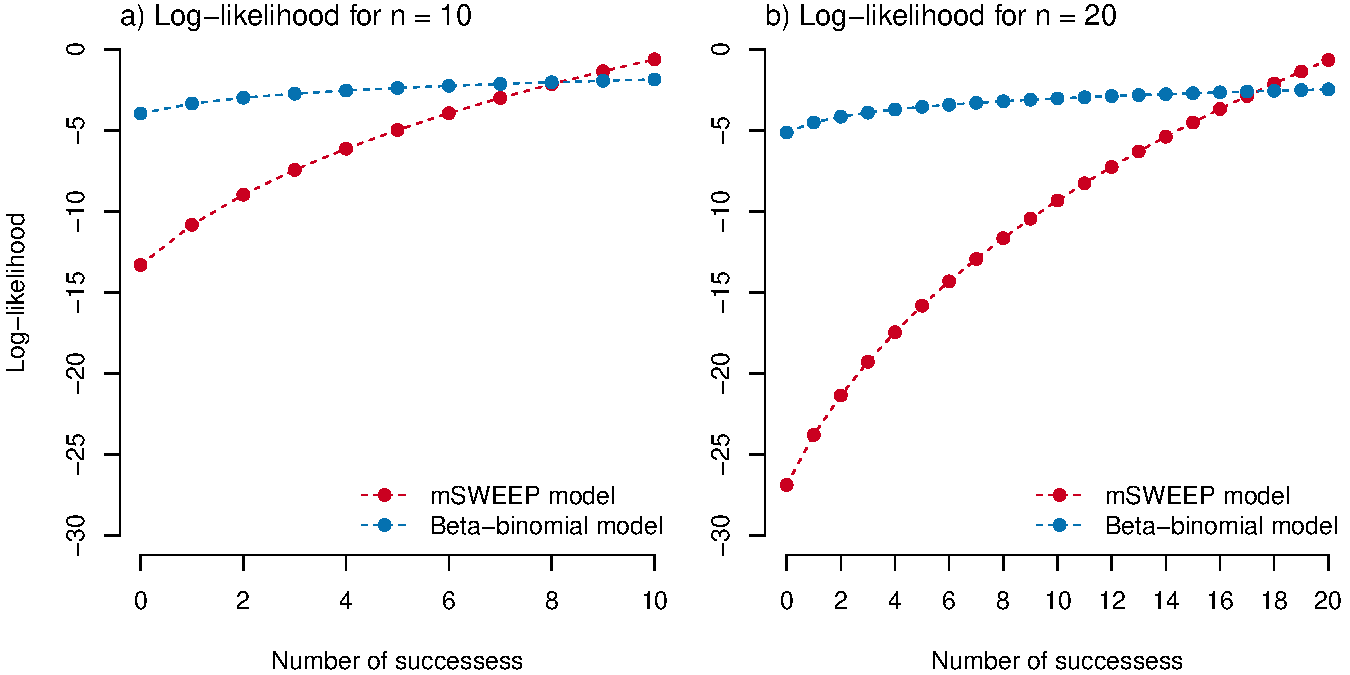
\includegraphics[width=\textwidth,keepaspectratio]{img/mSWEEP_likelihood.pdf}
    \caption{Comparison of the mSWEEP likelihood and a plain beta-binomial likelihood (without zero inflation). The figure displays the difference between the modified beta-binomial likelihood that mSWEEP uses (red dots and lines) and a plain beta-binomial likelihood (blue dots and lines) with the same parameters. Panel \textbf{a)} displays the difference for a cluster with 10 reference sequences, and panel \textbf{b)} for a cluster with 20 reference sequences.}
\end{figure}

A comparison of the likelihood presented in Equation
\ref{likelihood:beta-binomial-scaled} with the plain beta-binomial
likelihood in Equation \ref{likelihood:beta-binomial-pmf} is presented
in Figure \ref{fig:msweep-vs-beta-binomial}. Figure
\ref{fig:msweep-vs-beta-binomial} shows that the mSWEEP format gives
more weight to values of $k$ that are close to $n$ while making the
differences between the different $k$ steeper than the plain
beta-binomial. In practice, the modified format implies that the
clusters should be defined in a way that most reads will pseudoalign
to the cluster if the read originated from the cluster.

With the probability mass function of the distribution
$p^{\star}\left(k \middle| n, \alpha, \beta\right)$, the full
definition for the third part of the likelihood in Equation \ref{likelihood:without-normalization} is
\begin{equation}
  \label{likelihood:normalized}
  p\left(r_{n, k} \middle| I_{n} = k\right) = 0.99\frac{p^{\star}\left(r_{n, k} \middle| M_{k}, \alpha, \beta\right)}{Z\left(r_{n}\right)}\text{ if } r_{n, k} \geq 1\text{ and } M_{k} > 1,
\end{equation}
where $Z\left(r_{n}\right)$ is a normalizing constant that depends on
all observed pseudoalignment counts $r_{n, k}, k = 1, \dots, K$. The
scaling in Equation \ref{likelihood:beta-binomial-scaled} fulfills our
requirement that the likelihood of each cluster must be on the same
scale despite different size. The next section will derive a closed
form for the normalizing constant $Z\left(r_{n}\right)$.

\subsection{Normalizing the likelihood}

Although the function $p^{\star}\left(k \middle| n, \alpha,
\beta\right)$ in Equation \ref{likelihood:beta-binomial-scaled}
closely resembles the probability mass function of a Beta-Binomial
distribution (Equation \ref{likelihood:beta-binomial-pmf}), the
function $p^{\star}$ itself does not sum to $1$ over its support $k
\in \left\{ 1, \dots, K \right\}$. In order to turn the $p^{\star}$:s
into proper probability mass functions, we need the normalizing
constant $Z\left(r_{n}\right)$.

Although any distribution on a finite support can be normalized (TODO
citation), in many cases the normalizing constant does not have a
closed form. In our case it turns out that \textemdash thanks to the
properties of the beta function (see Equation
\ref{likelihood:beta-function} for the definition) \textemdash 
$Z\left(r_{n, k}\right)$ has a closed form. To derive the closed form,
we need the following identity for the beta function
\begin{theorem}
  \label{lemma:beta-function-identity}
  \[
  B\left(a + 1, b\right) = \frac{a}{a + b}B\left(a, b\right).
  \]
\end{theorem}

\begin{proof}
  Follows from $B\left(a, b\right) = \frac{\Gamma\left(a\right)\Gamma\left(b\right)}{\Gamma\left(a + b\right)}$ \citep{artin_einfuhrung} and $\Gamma\left(z + 1\right) = z\Gamma\left(z\right), \text{ for all } z > 0$ \citep{davis_leonhard}, where $\Gamma\left(z\right)$ is the gamma function. Using these two identities, we can write $B\left(a + 1, b\right)$ as
  \begin{align*}
    B\left(a + 1, b\right) &= \frac{\Gamma\left(a + 1\right)\Gamma\left(b\right)}{\Gamma\left(a + b + 1\right)} \\
    &= \frac{a\Gamma\left(a\right)\Gamma\left(b\right)}{\left(a + b\right)\Gamma\left(a + b\right)} \\
    &= \frac{a}{a + b}B\left(a, b\right).
  \end{align*}
\end{proof}

Using Lemma \ref{lemma:beta-function-identity}, we can find a closed form for the normalizing constant $Z\left(k\right)$.
\begin{theorem}
  \label{theorem:likelihood-can-be-normalized}
  Let
  \[
  f\left(k, n_{k}\right) = \binom{n_{k}}{k}\frac{B\left(\alpha + k, n_{k} - k + \beta\right)}{B\left(\alpha + n_{k}, \: \beta\right)}, 0 < k < n_{k}, \: \alpha > 0, \: \beta > 0,
  \]
  and
  \[
  Z\left(r_{n}\right) = \prod_{k = 1}^{K}Z\left(n_{k}\right) = \prod_{k = 1}^{K}\prod_{j = 1}^{n_{k}}\frac{\alpha_{k} + n_{k} + k - j}{\alpha_{k} + \beta_{k} + 2n_{k} - j},
  \]
  then TODO check after formulating the likelihood somewhere properly
  \[
  \sum_{k = 1}^{K} \frac{f\left(k, n_{k}\right)}{\prod_{k = 1}^{K}Z\left(n_{k}\right)} = 1.
  \]
\end{theorem}

\begin{proof}
  Consider a Beta-Binomial distribution with the parameters $\left(n, \alpha + n, \beta\right), n \in \mathbb{N}_{0}, \alpha > 0, \beta > 0$. This distribution has the probability mass function $g : 0, \dots, n \rightarrow \left[0, 1\right]$, where
  \[
  g\left(k \: \middle| \: n, \alpha + n, \beta\right) = \binom{n}{k} \frac{B\left(\alpha + n + k , n - k + \beta\right)}{B\left(\alpha + n, \beta\right)},\: 0 \leq k \leq n.
  \]
  Using the identity $B\left(a + 1, b\right) = B\left(a, b\right)\frac{a}{a + b}, a > 0, b > 0$ (Lemma \ref{lemma:beta-function-identity}) we can derive an alternative form for $g$:
\begin{align*}
  g\left(k\right) &= \binom{n}{k} \frac{B\left(\alpha + n + k , n - k + \beta\right)}{B\left(\alpha + n, \beta\right)} \\
  &= \binom{n}{k} \frac{B\left(\alpha + n + k - 1 , n - k + \beta\right)}{B\left(\alpha + n, \beta\right)} \frac{\alpha + n + k - 1}{\alpha + n + k - 1 + n - k + \beta} \\
  &= \binom{n}{k} \frac{B\left(\alpha + n + k - 1 , n - k + \beta\right)}{B\left(\alpha + n, \beta\right)} \frac{\alpha + n + k - 1}{\alpha + \beta + 2n - 1} \\
  &= \binom{n}{k} \frac{B\left(\alpha + n + k - 2 , n - k + \beta\right)}{B\left(\alpha + n, \beta\right)} \frac{\alpha + n + k - 1}{\alpha + \beta + 2n - 1} \frac{\alpha + n + k - 2}{\alpha + \beta + 2n - 2} \\
  &= \binom{n}{k} \frac{B\left(\alpha + n + k - 2 , n - k + \beta\right)}{B\left(\alpha + n, \beta\right)} \prod_{j = 1}^{2} \frac{\alpha + n + k - j}{\alpha + \beta + 2n - j}.
\intertext{Repeadetly applying Lemma \ref{lemma:beta-function-identity} $n$ times yields}
  g\left(k\right) &= \binom{n}{k} \frac{B\left(\alpha + n + k - n , n - k + \beta\right)}{B\left(\alpha + n, \beta\right)} \prod_{j = 1}^{n} \frac{\alpha + n + k - j}{\alpha + \beta + 2n - j} \\
  &= \binom{n}{k} \frac{B\left(\alpha + k , n - k + \beta\right)}{B\left(\alpha + n, \beta\right)} \prod_{j = 1}^{n} \frac{\alpha + n + k - j}{\alpha + \beta + 2n - j} \\
  &= f\left(k, n\right) \prod_{j = 1}^{n} \frac{\alpha + n + k - j}{\alpha + \beta + 2n - j}.
\end{align*}
Since $g\left(k\right)$ is a probability mass function, this implies that
\[
f\left(k, n\right)\left(\prod_{j = 1}^{n}\frac{\alpha + n + k - j}{\alpha + \beta + 2n - j}\right)^{-1}
\]
is also a probability mass function. Furthermore, since the products of (independent) probability mass functions are probability mass functions, then
\[
\prod_{k = 1}^{K}f\left(k, n_{k}\right)\left(\prod_{j = 1}^{n}\frac{\alpha + n_{k} + k - j}{\alpha + \beta + 2n_{k} - j}\right)^{-1}
\]
is also a probability mass function. Thus, since we assumed that the reads $r_{n}$ are independent of each other, setting
\[
Z\left(r_{n}\right) = \prod_{k = 1}^{K} \prod_{j = 1}^{n_{k}}\frac{\alpha_{k} + n_{k} + k - j}{\alpha_{k} + \beta_{k} + 2n_{k} - j}
\]
is sufficient to normalize $f\left(r_{n, k}, n_{k}\right)$ and prove Theorem \ref{theorem:likelihood-can-be-normalized}.
\end{proof}

\subsection{Likelihood hyperparameters}

Insteda of the traditional parametrization for the beta binomial
distribution through $\alpha >0, \beta > 0$, we use a
reparametrization that slightly changes the interpretation of the
parameters. The transformed parameters are
\begin{equation}
  \label{likelihood:reparametrization}
  \pi = \frac{\alpha}{\alpha + \beta}, \phi = \frac{1}{\alpha + \beta},
\end{equation}
where the first parameter $\pi$ has the range $\pi \in \left(0,
1\right)$ and represents the mean success rate in repeated draws from
the beta binomial distribution (TODO cite). The second parameter $\phi
> 0$ measures the variation in the success rate for each draw. In our
formulation for the likelihood, each cluster $k$ has its own
parameters $\pi_{k}, \phi_{k}$.

Although methods such as Bayesian optimization (TODO cite) could
be employed to find optimal values for the parameters $\pi_{k}, \phi_{k}$ in
Equation \ref{likelihood:reparametrization}, we set their values based
on a nonexhaustive analysis on several data sets (TODO explain). The
values of $\pi, \phi$ are set to
\begin{equation}
  \begin{aligned}
    \pi_k &= 0.65, \text{ for all } k = 1, \dots, K, \\
    \phi_{k} &= 1 - \pi_{k} + 0.01M_{k}^{-1}.
  \end{aligned}
\end{equation}
Next, we show that slightly varying the values does not significantly
affect the results of the analyses.

TODO experiment on the mGEMS paper data about varying the
hyperparamter values.

- hyperparameters - may be add a sensitivity test?

\subsection{Fitting the model using variational inference}

With the likelihood defined in Equations
\ref{likelihood:without-normalization} and
\ref{likelihood:normalized}, all that remains is to come up with a
suitable method to infer the relative abundances
$\boldsymbol\theta$. Since our model is principally the same as the
one used in BIB (Equation \ref{model:grouped-joint-distribution}),
just with a different formula for the likelihood term $p\left(r_{n, k}
= k \middle| I_{n} = k\right)$, we can adapt the variational inference
used in BIB to our needs. Since this requires only changing the
likelihood term, the core of the inference algorithm remains the
same. Since variational inference is an extremely broad topic outside
of the scope of this dissertation, I will only cover the parts that
are relevant to the original contributions in the thesis. For a more
thorough coverage of the variational inference algorithm, readers are
referred to TODO (cite VI papers), which cover the variational
inference in detail, and TODO (cite gradu) which contains a summary of
the applicable parts from the previous papers in the context of this
model but with a slightly different format for the likelihood.

In brief, variational inference for the mSWEEP model consists of
finding a distribution $q\left(\boldsymbol\theta, I\right)$ that
minimizes the Kullback-Leibler divergence to the true posterior
$p\left(\boldsymbol\theta, I \middle| R\right) \approx
q\left(\boldsymbol\theta, I\right)$. For simplicity, we assume that
the approximation $q\left(\boldsymbol\theta, I\right)$ factorizes into
$q\left(\boldsymbol\theta, I\right) =
q\left(\boldsymbol\theta\right)q\left(I\right)$. Since we assumed that
each $I_{n}$ has a categorical distribution
$Cat\left(\boldsymbol\theta\right)$ and are independent of each other,
$I_{n} \indept I_{m}, n \neq m$, the second term $q\left(I\right)$
simplifies to
\begin{equation}
  \label{likelihood:vi-factorization}
  q\left(I\right) = \prod_{n = 1}^N\prod_{k = 1}^K \gamma_{n, k}^{I_{n, k}}.
\end{equation}

In practice, the best approximation $q\left(\boldsymbol\theta,
I\right)$ is found when optimal values for the parameters $\gamma_{n,
  k}$ in Equation \ref{likelihood:vi-factorization} are found (TODO
cite). We use the Riemannian conjugate gradient (RCG) method to find
the optimal values for $\gamma_{n, k}$ (TODO cite). A generic and
parallel \& distributable implementation for arbitrary likelihood with
this mixture model structure is available from
\url{https://github.com/tmaklin/rcgpar}.

\subsection{Alternative fit using MCMC sampling}
Alternatively, the model could be fitted using Markov chain Monte
Carlo (MCMC) sampling methods (TODO citations or explain). Instead of
finding an approximating distribution $q\left(\boldsymbol\theta,
I\right)$, MCMC sampling attempts to produce a set of samples from the
true posterior $p\left(\boldsymbol\theta, I\middle|
R\right)$. Averaging over the values produced via MCMC sampling
$\hat{\boldsymbol\theta}$ asymptotically produces the true parameters
$\boldsymbol\theta$ as the number of samples $n_{MCMC}$
increases. Even though producing the true values is tempting instead
of using the values from the variational approximation, MCMC has
several problems when applied in practice (TODO citations). First, the
true values are only found asymptotically, meaning that it is
difficult to measure when the sampling has been performed for long
enough for the chain to have converged to the true
posterior. Secondly, due to the first point, the number of samples
that need to be drawn may be excessively high, resulting in extremely
long run times when compared to the faster variational inference (TODO
cite).

MCMC does however have the advantage that, provided sufficient
runtime, the samples will be from the true posterior. When comparing
MCMC to VI in practice, the former has been reported to better capture
correlations between the sampled parameters (TODO cite Antti's bitseq
paper). Because of this, we compared the VI from mSWEEP to a version
of mWEEP compatible with the MCMC sampling from BitSeq (TODO cite
BitSeq) but found no significant differences between the two (TODO figure).

- Add results from Gibbs sampler vs variational inference experiments.

\section{From profiling to binning}
\label{section:binning}

This sections covers using the model from mSWEEP to provide an
algorithm for binning sequencing reads. Binning differs from the
abundance estimation, or taxonomic profiling, in that the goal is to
produce some assignment of the reads to reference units. In typical
cases, bins correspond to some individual species or genuses, but in
this thesis binning will be performed on the level of the clusters
that mSWEEP uses for reporting the relative abundances. Compared to
merely doing taxonomic profiling, binning provides a much higher level
of detail about the contents of a sample, since many read-based
downstream analyses may be performed once the bins have been
constructed. Contrary to the section presenting the probabilistic
model, the binning algorithm is quite straightforward.

The work in this section is based on the results from the second paper
included in the dissertation \citep{maklin_bacterial_2021}.

\subsection{The mGEMS binning algorithm}

A crucial feature for the binning algorithm to handle lineage-level
differences between bacteria is the possibility for a single read to
belong to multiple bins at the same time. This differs from most of
the work on binning, where the reads are typically only assigned to a
single bin and the variation between the bins is assumed large enough
that this approach is correct. For strain-level-binning to work, this
assumption is obviously not correct, since the differences between the
genomes can be minimal. Thus, the binning algorithm must be derived
with this feature in mind.

The mGEMS binning algorithm is derived by leveraging the read-level
assignment probabilities $\gamma_{n, k} \in \left(0, 1\right), n = 1,
\dots, N, k = 1, \dots, K, \sum_{k = 1}^{K}\gamma_{n, k} = 1$ produced
by the variational approximation (Equation
\ref{likelihood:vi-factorization}). We assume that the sequencing
reads do not contain several members of the same cluster and that,
should the true reference sequence that generated the reads be missing
from the reference, the set of reference sequences adequately captures
the variation present in the cluster. To fulfill our requirement that
the read can belong to several bins at the same time, we define a bin
$G_{k}$ for each cluster $k$ as a subset of sequencing reads $r_{n}$
such that
\begin{equation}
  \label{binning:bins-definition}
  G_{k} = \left\{r_{n} : \gamma_{n, k} \geq q_{k}\right\}
\end{equation}
holds for a threshold $q_{k} \in \left[0, 1\right]$. The threshold may
be different for each cluster $k$. Because of the way the bins $G_{k}$
are defined in Equation \ref{binning:bins-definition}, this definition
obviously allows for the reads to belong to several bins (for a
trivial example, consider the case where $q_{k} = 0$ for all $k$).

\subsection{Assignment rule for multi-cluster membership}

Next, we need to find a sensible value for the thresholds $q_{k}$ that
ideally maximizes the probability $A_{n, k}$ of assigning the read
$r_{n}$ to the bin $G_{k}$ if the cluster $k$ (could have) generated
the read $r_{n}$. Ideally, we would define the probability $A$ through
another probability $B_{n, k}$: the cluster $k$ contains a sequence
that contains the true (error-free) nucleotide sequence of the read
$r_{n}$. However, the probability $B$ is difficult to estimate
directly since 1) the reads cannot be error-corrected with full
accuracy, and 2) the reference collection is non-complete. However, by
assuming that the sample is composed mostly of closely related
organisms, we can derive the following relationships between $A_{n,
  k}$ and $B_{n, k}$
\begin{equation}
  \label{binning:a-is-approximately-b}
  P\left[A_{n, k} = 1\right] \approx \theta_{k}P\left[J_{n, k} = 1\right],
\end{equation}
where $\theta_k$ is the relative abundance of the cluster $k$ in the
sample that generated the reads $r_{n}$. Equation
\ref{binning:a-is-approximately-b} implies that when $P\left[A_{n, k}
  = 1\right] \geq \theta_{k}$, then $P\left[B_{n, k} = 1\right]$ must
be ``large'' for the approximation to hold. A more detailed derivation
for this statement about the magnitude of $B_{n, k}$ and Equation
\ref{binning:a-is-approximately-b} is provided in the methods section
of the mGEMS article \cite{maklin_bacterial_2021}, supplied in the
appendix for this thesis, and thus omitted from here.

The implied statement about the magnitude of $B_{n, k}$ when
$P\left[A_{n, k} = 1\right] \geq \theta_{k}$ means that there is a
high chance that $B_{n, k} = 1$ when the former holds. Through this,
we can derive an assignment rule by using the estimates $\gamma_{n,
  k}$ (Equation \ref{likelihood:vi-factorization}) for the probability
$P\left[A_{n, k} = 1\right]$
\begin{equation}
  \label{binning:theoretical-assignment-rule}
  \text{if } \gamma_{n, k} \geq \theta_{k}, \text{ assign the read } r_{n} \text{ to } G_{k}.
\end{equation}
Equation \ref{binning:theoretical-assignment-rule} provides us with an
inequality whose validity can be checked to assess the probability of
the event $B_{n, k} = 1$ which we could not estimate directly.

\subsection{Practical considerations}

While the assignment rule in Equation
\ref{binning:theoretical-assignment-rule} provides a theoretically
sound tool to assign reads $r_{n}$ to the bins $G_{k}$, applying it in
practice requires a slight adjustment due to computational
accuracy. Namely, when estimating the relative abundances $\theta_{k}$
of $N$ reads, any estimate that falls below $\frac{1}{N}$ means that
zero reads originated from the cluster $k$. Because of this, values
$\theta_{k} < \frac{1}{N}$ are meaningless and all represent the same
case of 0 reads from the cluster. Due to the constraint that
$\theta_{k}$ must sum up to $1$ over $k$, these essentially-zero
values do, however, contribute a small amount of noies to the
estimates. Since there are $K$ clusters, the fraction of noise $d$ is
(in the worst-case scenario) at most
\begin{equation}
  \label{binning:assignment-rule-noise}
  d = K\frac{1}{N}.
\end{equation}

Equation \ref{binning:assignment-rule-noise} means that when
evaluating the validity of the inequality presented in Equation
\ref{binning:theoretical-assignment-rule}, we should adjust the
threshold $\theta_k$ with $1 - d$, meaning that we consider only the
fraction of relative abundance that is assigned to nonzero
estimates. This produces the final assignment rule that is used in
mGEMS
\begin{equation}
  \label{binning:assignment-rule}
  \text{if } \gamma_{n, k} \geq (1 - d)\theta_{k}, \text{ assign the read } r_{n} \text{ to } G_{k}.
\end{equation}

Since the variational approximation used to fit the mSWEEP model
already provides both the estimates $\gamma_{n, k}$ and the relative
abundances $\theta_{k}$, the assignment rule in Equation
\ref{binning:assignment-rule} is in practice extremely inexpensive to
evaluate after the model has been fitted.

Since the relative abundances $\theta_k$ are derived from the values
$\gamma_{n, k}$ by averaging over $n = 1, \dots, N$, the assignment
rule in Equation \ref{binning:assignment-rule} can be seen as a way to
cluster the rows (or columns) of a generic probability matrix while
allowing assigning each row (or column) to several clusters at the
same time. We do not, however, explore the applicability of this rule
to other scenarios where a probability matrix should be clustered in
this manner. Nevertheless, the rule is general enough to acknowledge
its potential applications elsewhere.

The next chapter will cover the application of mSWEEP and mGEMS to
both different kinds of sequencing data and explore how the methods
can be applied to enable new directions in analysis of sequencing
data. The chapter also includes a brief coverage of the benchmarks and
experiments presented in the first and second papers (TODO cite).

\chapter{High-resolution metagenomics}

High-resolution metagenomics (in the context of this thesis) refers to
applying some method capable of recovering variation at the
within-species level to some sort of metagenomics data as defined in
Section \ref{three-approaches-to-metagenomics}. In our case, the
methods of interest are mSWEEP and mGEMS. This chapter will deal with
the benchmarking and experimental results from the first two papers,
which focus on analysing plate sweep metagenomics data. At the end of
the chapter some technicalities arising from the model formulatin will
also be covered \textemdash namely questions about reliability of the
results when applied to realistic use-cases and sensitivity to
parameter changes.

\section{Plate sweep and WGS metagenomics}

The primary methods for obtaining metagenomics sequencing data
considered in this thesis are plate sweep metagenomics and
whole-genome shotgun (WGS) metagenomics (see Section
\ref{three-approaches-to-metagenomics} for more details). Of these
two, plate sweep metagenomics has the advantage of being able to focus
sequencing efforts to species that are known to grow on specific
plates, while WGS metagenomics provides data of \textit{all} organisms
on some sample (including for example host DNA, fungi, commensal
species). When the goal is to investigate strain-level variation, both
approaches have their uses in either producing more data from the
species of interest or providing a less biased view of the sample
contents at the expense of sequencing depth. The first two papers
included in the thesis were written with only plate sweep metagenomics
in mind but the third paper demonstrated that mSWEEP and mGEMS are
applicable in the WGS metagenomics context. Thus, this chapter will
not discriminate between the two.

\subsection{Benefits of metagenomics over culturing}

When comparing metagenomics approaches to culturing, the obvious
difference is that the former will provide a better view of the
microbiome in the sample. Although epidemiological analyses in the
past have mostly focused on using isolate data, some studies showing
the benefits of using a metagenomics approach have emerged. In
particular, a recent study utilizing mSWEEP and mGEMS showed that
using isolate sequencing data alone can result in an approach that
dismisses the presence of non-dominant variants of the same species
\citep{tonkin-hill_pneumococcal_2022}. Similar approaches using other
tools have also hinted at the capability of several strains to become
pathogenic should the opportunity present itself (TODO
citations). These studies have demonstrated that it may be necessary
to incorporate some level of metagenomics in epidemiological studies
in order to better identify the causative agents (TODO citations) of
disease.

Microbiome studies in general have become increasingly popular with
the advent of 16S sequencing. Although the results of some studies
remain somewhat controversial, the widespread application of this
method has revealed extensive variation in the microbiome contents
sampled form comparable sources. It is currently an open question
whether this variation extends to the strain-level but nevertheless
there exist studies both old and new that suggest this to be the
case.

mSWEEP and mGEMS specifically enable answering questions about
strain-level variation by providing a method that can be targeted to
identify the variation in some species. Since many species of clinical
importance have been studied for several decades with significant
sequencing efforts aimed at them to obtain high-quality genome
assemblies, the reference-based approach employed by mSWEEP and mGEMS
is ideal for disentangling variation in the same setting. When
combined with tools with other kinds of approaches to sequencing, the
methods together have the potential for unprecedented level of detail
in epidemiologic analyses and tracking

While the previous chapter covered the theoretical foundations of
mSWEEP and mGEMS, the rest of this chapter will focus on evaluating
some practical considerations regarding the methods. Namely, we
briefly overview the performance of the methods when compared to other
established approaches, and cover some questions related to the
reliability of the approach as well as the sensitivity to the
parameter choices. The last part of the chapter will cover some
results from the included papers related to what kind of information
metagenomics-derived results provide.


\subsection{The mSWEEP/mGEMS pipeline}

- Flowchart describing the analysis pipeline.

Combining the results from Sections \ref{section:model} and
\ref{section:binning} produces the complete workflow for analysing
sequencing data from mixed sources. This workflow is originally
presented in the second paper \citep{maklin_bacterial_2021}, where it
is referred to as the mGEMS pipeline.

\subsubsection{Constructing the reference database}

The pipeline begins with constructing a set of reference sequences
that represent the variation in the target species of interest. In an
ideal scenario, the reference should consist of high-quality
assemblies from each lineage that is expected to be found in the
sequencing reads. Since this is a rather unrealistic assumption,
typical cases make use of published datasets and possible combine
isolate sequencing data from their own studies. Either previously
published assemblies or even curated genomes from databases such as
RefSeq may be used but the reference may also include newly assembled
sequences or otherwise be tailored to the problem at hand. In both
cases a cautious approach is recommended, as the quality of the
reference sequence set is the most important factor in obtaining
trustworthy results from the pipeline.

After the appropriate reference sequences have been collected, they
should be clusered in some meaningful way to obtain the grouping. For
some species, multilocus sequence typing is sufficient but for others
with more variable genome contents, algorithms that attempt to
identify clonal complex analogues may be uesful. One such algorithm is
PopPUNK, which is demonstrated to perform relatively well in the third
paper included in this thesis. PopPUNK clusters the reference
sequences based on accessory and core genome distances, and provides
results that are very similar to clonal complexes (groups of STs) for
species where the complexes are defined. Using a computational like
PopPUNK instead of a curated database approach like sequence types and
clonal complexes has the advantage of being able to assign sequences
that have not yet been included in the curated databases, or work with
species for which such databases do not exist.

After clustering the reference sequences, the next step is to build an
index for pseudoalignment, and pseudoalign the reads from the samples
against the index. In the mGEMS pipeline, we use Themisto to perform
both the index construction and the pseudoalignment. The
pseudoalignment step produces the alignment vectors for each read
against every reference sequence, which are used as the input to
mSWEEP.

\subsubsection{Estimating relative abundances and binning the reads}

The next step in the pipeline is to use mSWEEP to estimate the
relative abundances of the reference groups based on the
pseudoalignments against the sequences. This is performed directly on
the output from Themisto, with no intermediate steps required. After
the relative abundances have been estimated, the results are fed to
mGEMS which produces the read bins and optionally also extracts the
reads corresponding to each bin from the original set.

\subsubsection{Assembling the read bins}

In the second article of this thesis, the mGEMS pipeline also includes
an optional step to assemble the sequences. The suggested assembler is
shovill, which is an assembly pipeline built around the spades
assembler but incorporating some pre- and postprocessing
steps. Naturally other assemblers may also be used, or the assembly
step skipped entirely and the analysis instead focusing the reads. In
the second article we mostly focused on analysing the assemblies, as
including an assembly step introduces a postprocessing step that can
be useful in filtering out reads that have been mistakenly assigned to
the bin.

Since mGEMS allows for including a sequencing read in several bins at
once, the produced read bins may have a very high coverage for shared
parts of the genome when the sample contains several closely related
organisms. Because of this, we investigated the effect of replacing
the isolate-data optimised shovill with metagenomic assemblers, which
presumably implement better handling of variable coverage in the
produced genomes. Although we observed some differences in the
resulting assemblies, there was no statistically significant evidence
in favour of using either approach. Regardless of the assembler
choice, using the mGEMS pipeline produced assemblies in downstream
analyses performed similarly to a benchmark consisting of assemblies
derived from isolate sequencing data.

\subsubsection{Quality control}

The mGEMS pipeline as described above is the method that has been
applied in the third paper with the additional inclusion of a
postprocessing step aimed at identifying whether the reference
sequences suitably cover the reads or not. This postprocessing step,
demix\_check (\url{https://github.com/harry-thorpe/demix_check/}),
performs several quality control checks on the results from mSWEEP and
mGEMS, aiming to determine whether the created read bins correspond to
a reference cluster or not. Although this step was not included in the
two methods papers presenting mSWEEP and mGEMS, its inclusion
addressess an important question regarding the applicability of the
results from mSWEEP/mGEMS. Therefore, including demix\_check
\textemdash or other similar approach \textemdash as part of the mGEMS
pipeline (between the mGEMS and the assembly steps) is recommended for
a rigorous approach. This and other questions related to quality
control and reliability of the results are explored further down in
this chapter.

- figure from presentation showing the threshold construction process.

\subsection{Other approaches for metagenomic analyses}
\label{other-metagenomics-approaches}
While this thesis deals with the development and usage of mSWEEP and
mGEMS, one has to acknowledge that the use of metagenomic sequencing
data is by no means an understudied field. In fact, dozens of methods
exist that aim to perform similar tasks ranging from genome assembly
from metagenomic sequencing data (metagenome assemblers) to taxonomic
binning (metagenomic binners) and profiling, and strain tracking
(StrainGE and Strainphlan). Compared to mSWEEP and mGEMS, these
methods typically assume that the samples only contain a single strain
from each species, which makes the task solvable. While it may at
first seem suspicious that a thorough comparison between these methods
and mSWEEP/mGEMS has not been included in the published papers, the
assumptions about the strain complexity lie at the heart of the
problem. Since these tools have not been developed with the kind of
data that mSWEEP/mGEMS analyse in mind, a performance comparison
between them is not meaningful.

\section{Benchmarking mSWEEP and mGEMS}
This section will briefly cover the results related to benchmarking
the performance of mSWEEP and mGEMS in the first and the second
papers. A majority of the benchmarks were performed on synthetic
mixtures of sequencing reads from isolate cultures but the mGEMS paper
also provides a (significantly smaller in scale) benchmark that used
\textit{in vitro} mixtures of DNA from isolate cultures. Figures from
the papers have not been reproduced here, and the results are
presented in a summarizing format merely to convince the reader of the
kinds of applications that mSWEEP and mGEMS perform well in.

\subsection{mSWEEP}
The first paper in the thesis presented a comparison of mSWEEP with
the Bayesian Identification of Bacteria (BIB) and the
pseudoalignment-based metakalisto methods. Although a myriad of
taxonomic profilers have been developed (these will be covered in more
detail in Section \ref{other-metagenomics-approaches}), the vast
majority of them do not attempt within-species profiling or have been
developed for cases with only one strain present from each
species. Because of these limitations, the mSWEEP paper only makes the
comparisons with BIB and metakallisto, which claim to work in a
setting with several strains present.

TODO something about how BIB and metakallisto work

The main result of the first paper is that mSWEEP vastly outperforms
both BIB and metakallisto for most species. For species with a
strictly defined clonal structure \textemdash such as
\textit{S. aureus} \textemdash, BIB and metakalisto are able to derive
comparable performance, but for other species that exhibit more varied
clonal structures incorporating the probabilistic model from mSWEEP
proves to be a necessary step in obtaining accurate
information. Although these performance benchmarks were only performed
on data containing a single strain in each sample, we demonstrate in
the paper through stochastic dominance that the methods which do not
succeed with single-strain estimates are unlikely to provide accurate
results from multi-strain samples.

Another benchmark presented in the first paper concerns evaluating
performance in the presence of several strains from the same
species. In this benchmark, sequence data from three strains were
mixed together in single sample at known proportions, and mSWEEP was
applied to estimate the proportions when the real reference sequences
were absent from the reference data but close representatives from the
same lineage were available. In this benchmark, mSWEEP demonstrates
very accurate performance measured on both true positives and true
negatives. Although \textit{K. pneumoniae} in particular proved
challenging, possibly due to the wide variety exhibited in the
reference set, the results were nevertheless within acceptable error

In addition to the synthetic experiments presented in the first paper,
the second paper presents an \textit{in vitro} benchmark concerning
abundance estimation. In this benchmark DNA from three different
strains of either \textit{E. coli} or \textit{E. faecalis} was mixed
together using Qbit, producing samples where the initial composition
of the sample is known at the DNA level. This benchmark shows similar
results as the synthetic benchmarks for \textit{E. faecalis}, where
the three strains originated from three different sequence types, but
also shows promise in differentiating between strains of the same
clade within a single sequence type of \textit{E. coli}. This task is,
however, much, much more difficult since the split of the ST131
subclade C2 was based on incorporating information from the accessory
genome using PopPUNK. The accessory genome of \textit{E. coli} is not
as stable as the core genome, on which the ST131 and the ST131 A-C
designations are based, resulting in some difficulties in separating
the C2-4 and C2-6 sublineages. Nevertheless mSWEEP manages to identify
the presence of both clades quite well, and the downstream analysis
using mGEMS (covered in Section \ref{mgems-performance-benchmark}
still provides accurate results.

\subsection{mGEMS}
\label{mgems-performance-benchmark}

Our taxonomic binner mGEMS was benchmarked in the second paper using
both synthetic data (mixtures of reads from isolate cultures of
different strains) as well as the previously mentioned \textit{in
  vitro} benchmark. The chief metrics used were related to those that
are the main objects of interest in genomic epidemiological analyses:
SNPs and phylogenies estimated from the SNP data. We looked at the
performance of mGEMS on the level of within-ST variation using data
from \textit{E. coli} (TODO cite paper), at the between-ST and
within-species level using \textit{E. faecalis}, and an extreme case
with only dozens of SNPs separating the different reference clusters
using data from \textit{S. aureus}.

\subsubsection{Synthetic data benchmarks}

In the \textit{E. coli} benchmark we investigated how well
mGEMS-derived assemblies performed for maximum likelihood phylogeny
estimation (using RAxML-NG, Gamma+GTR4M model) when compared to using
isolate sequencing data. We used snippy to derive the core genome
alignment against the same reference genome for both mGEMS-derived
assemblies and the isolate assemblies. The results showed that mGEMS
tends to slightly overestimate the number of SNPs in these assemblies
(Figure 2 panel a in the paper (TODO cite)) but the phylogenetic
relationships (Figure 3) are recovered quite well. This benchmark was
performed at the level of variation within a sequence type
(\textit{E. coli} ST131).

The \textit{E. faecalis} benchmark was performed similarly to the
\textit{E. coli} one but with the intention of investigating
performance with between-ST variation. Additionally,
\textit{E. faecalis} is known to have a relatively high rate of
recombination within the species across ST lines (TODO citation),
which adds to the difficulty of the problem. Nevertheless, the mGEMS
derived-assemblies do recover the overall structure of the phylogeny
and place to sequences from the same ST to the same clade. While the
global structure is somewhat different from the isolate assembly
phyolgeny, these kind of differences may easily be explained by
uncertainty arsing from recombination affecting the placement of the
STs globally. This phenomenon is also apparent in the bootstrap
support values for both the isolate and mGEMS-derived phylogenies.

The final synthetic benchmark in the second paper investigated
phylogeny recovery in \textit{S. aureus} ST22 sublineages that are
separated by a few dozen SNPs (TODO citation). Although the
performance in this benchmark was not quite as good as in the two
others, the mGEMS-derived results nevertheless do manage to replicate
some parts of the results relating to the transmission analysis
performed in the source study for this data. Namely, the samples that
were observed to be the likely source of the pathogenic strain in the
sequenced patients were placed at the root of the phylogeny when using
both mGEMS and isolate data. Regardless, there is some lack of detail
further down in the tree which is likely a result of the small degree
of separation between the sublineages.

\subsubsection{\textit{In vitro} benchmark}

The second paper also included an \textit{in vitro} benchmark data,
where known amounts of DNA from three different strains were mixed
together using Qbit, and both the mixed sample and the corresonding
isolate cultures were sequenced. This data was used to re-test the
performance of both mSWEEP (covered in the previous subsection) and
mGEMS. The mGEMS part of the test examined the recovery of SNPs from
either the isolate sequencing data or the mixed sequencing data. In
both the \textit{E. coli} and \textit{E. faecalis} test samples the
SNPs recovered from the mGEMS data reflect the ``true'' values from
the isolate data quite closely, although there is some difficulty in
separating the ST131-C2 sublineages 4 and 6. However, due to the
increasingly difficult task of defining sublineages within
sublineages, this difficulty is likely not relevant for practical
analyses.

Together, these benchmarks hopefully show that the mGEMS method can be
reliably used to disentangle metagenomic sequencing data and create
lineage-specific read bins. These bins in turn can be used in standard
epidemiological analyses in place of isolate sequencing data,
producing similar results. While mGEMS does not completely replace the
use of isolate sequencing data in epidemiology \textemdash the
availability of high-quality reference sequences from isolate
sequencing remains a critical part of the pipeline \textemdash the
method nevertheless shows promise in reducing the number of isolate
cultures that need to be created. Additionally, applying mGEMS to pure
metagenomics sequencing data can yield results that previously
available tools have not been able to produce as will be shown in more
in Chapter \ref{section:metagenomic-epidemiology} that covers the
experimental results from the third paper.

\section{Assessing reliability of the results}

A principal question when applying mSWEEP/mGEMS in practice is whether
the results from either are trustworthy or not. Since the former
method uses a Bayesian approach to estimating the relative abundances
of the reference lineages, none of the abundances will ever be exactly
zero. This naturally results in the question: ``When is a lineage
truly present in the sample?'' when applying mSWEEP in
practice. Furthermore, since the abundance estimates from mSWEEP are
the basis for the mGEMS pipeline, it is of importance to know when the
results for lineages with a high (in some sense) relative abundance
are truly correct and not just a result of, for example, missing
reference lineages. These two questions will be covered in the rest of
this section.

\subsection{Detection thresholds for lineages}
To answer the question regarding the minimum abundance required to
call an abundance estimate reliable or not, the mSWEEP paper provides
an approach termed \textit{detection thresholds}. These thresholds aim
to provide a minimum abundance that the estimates must exceed in order
to be reliable, and give accompanying p-value-analogues to assess the
degree of trust in the threshold itself. Although this approach is
computationally somewhat cumbersome to apply in practice, especially
when the size of the reference sequence set increases, the approach
should nevertheless provide means for more careful consideration of
the estimates without resorting to simpler measures such as filtering
by a constant abundance.

The detection threshold approach is based on bootstrapping sequencing
reads from existing samples with known genome assemblies in the
reference collection. The assembly is removed from the reference, and
the bootstrapped reads (which contain data from only the single,
removed assembly) are put through mSWEEP to obtain a bootstrapped
abundance estimate. This approach is then repeated for some number of
reference sequences, each removed in turn, to provide several
bootstrapped abundance estimates for each reference lineage. The
bootstrapped estimates are used to evaluate the magnitude of the
relative abundance estimates that are given for the \textit{absent}
lineages, and combined across all values generated when varying the
removed reference sequences. When repeated for all reference lineages,
this approach gives a set of values that represent the false estimates
when the true contents of the sample are differen. The false estimates
for each lineage are ordered, and one of the higher values is picked
as a cutoff point that defines the detection threshold for this
lineage with an accompanying p-value-analogue that depends on the
number of estimates that are allowed to exceed the cutoff. This
somewhat complicated approach is described in more detail in the first
paper.

While the detection thresholds approach has some merit in its
theoretical foundations in using bootstrapping to estimate the
magnitude of the false estimates, the approach has some problems when
applied in practice. Namely, the need to remove a reference sequence
to bootstrap the abundance estimates necessitaes reconstruction of the
pseudoalignment index for each sample that is generated from the
removed sequences. Since dynamic indexing (meaning that sequences can
be added/removed without rebuilding the whole index) remains an open
problem at the time of writing, the approach is quickly rendered
computationally infeasible when applied to reference sets that are
larger than those used in the mSWEEP paper. Unfortunately for the
detection threshold construction, for many applications it is tempting
to include as much reference data as possible to cover naturally
occurring strain-level variation. This has resulted in the approach
being not applied in practice and remaining a curiosity until dynamic
indexes hopefully become available.

\subsection{Pseudocoverage as a threshold}

One alternative to the detection thresholds can be found by figuring
out a way to define some sort of threshold on the abundance estimates
without utilizing bootstrapping-based approaches. In practice, this
translates to using the number of aligned reads and the abundance
estimates together to estimate the \textit{pseudocoverage} of the
reference lineage. Pseudocoverage $c^{\star}_{k}$ for reference
lineage $k$ is defined as the product of the abundance estimate
$\theta_{k}$ for lineage $k$ and the total number of bases $b$ in the
reads that pseudoaligned against any reference sequence divided by the
average genome length $l_{k}$ in lineage $k$
\begin{equation}
  \label{pseudocoverage}
  c_{k}^{\star} = \frac{\theta_{k}b}{l_{k}}.
\end{equation}
Although the definition in Equation \ref{pseudocoverage} is similar to
the basic definition of average coverage (number of bases in aligned
reads divided by genome length), these two definitions are not
necessarily the same.

To elucidate the difference between coverage and pseudocoverage,
consider a set of sequencing reads originating from two bacterial
strains, both with $100$ base pair long genomes, that differ by a
single base pair and are present in equal proportions in the sample
providing the sequencing reads. Assuming that we have 100 one base
pair long reads from each position in both genomes, the average
coverage of both strains would be $199$ since $9900\cdot2$ reads
will align to both genomes and only $100\cdot2$ reads will align to
just one. However, when considering the relative abundance estimates
for these two strains, their true values are $0.50$ and $0.50$ since
we know that both strains are present in equal proportions. This gives
both strains a pseudocoverage of $99.5$ \textemdash a conservative
value compared to the traditional coverage definition.

Pseudocoverage can be used to define a threshold on the relative
abundance estimates by finding the value of $\theta_{k}$ that provides
for example a pseudocoverage of \textit{at least} $1$x. Since the
pseudocoverage is a conservative estimate of the true coverage (the
exact, typically more complex than in the thought experiment above,
relationship depending on the relatedness of the lineages $k$), this
minimum value can be taken as a sort of a threshold on the relative
abundances. If combined with means to investigate whether the lineages
that remain after filtering by this approach are a good fit to the
reference lineages, pseudocoverage provides an adjustable rule that is
more easy to evaluate than the detection thresholds described above.

\subsection{Compatibility of the clustering and the reads}
The remaining question regarding the reliability of the estimates from
mSWEEP concerns the fit of the reference lineages with the estimated
contents of the bins produced by mGEMS. This issue was not covered in
neither the mSWEEP nor the mGEMS paper but since the publication of
the first, an external method has been developed to address the
question. This method, called demix\_check (TODO citation), uses mash
(TODO citation) distances between the bins from mGEMS and the
reference sequences assigned to each lineage to evaluate the fit
between the read bin and the lineage. In practice, demix\_check has
proved invaluable in addressing the results from mGEMS and is an
integral part of the processing pipeline that was used in the third
paper of this thesis. Since this method was not developed by the
author of this thesis, it won't be covered in more detail although its
inclusion in the mGEMS pipeline is strongly recommended.

%% \subsection{Brief consideration of model assumptions}
%% %% * Not needed *
%%
%% For a reader more versed in probabilistic modelling, a final question
%% regarding reliability would relate to the assumptions made by the
%% mSWEEP model and when and whether those assumptions hold or not.
%%
%% - Zero inflation vs no inflation; degree of inflation
%% - Sensitivity to hyperparameter values

\chapter{Metagenomic epidemiology}
\label{section:metagenomic-epidemiology}

\section{Genomic epidemiology}

- describe what genomic epidemiology is
- descrie 
Something about wgs and genomic epidemiology can do lots of cool stuff
to identify contaminated cucumbers or track covid.

\section{From genomic to metagenomic}

\subsection{Using metagenomics-derived results}

- Stuff about how to interpret results from metagenomics

\subsection{Challenges}
- Challenges in using metagenomic data

\subsection{Advantages}
- Advantages of using metagenomic data

\section{Metagenomic epidemiology in practice}
\subsection{Plate sweep metagenomics}

Describe the experimental results from the first two papers.

\subsection{WGS metagenomics}

Describe the experimental results from the third paper.

\section{Future considerations}

\subsection{Applicability}
How do these show that what our methods are capable of and what they
could potentially be applied to in the future.

\subsection{Enables}
More speculative chapter.

\printbibliography[heading=bibintoc]

\chapter*{Included papers\markboth{Included papers}{}}
\addcontentsline{toc}{chapter}{Included papers}

\subsection*{Paper I \textemdash High-resolution sweep metagenomics using fast probabilistic inference}
By \underline{Tommi Mäklin}, Teemu Kallonen, Sophia David, Christine J
Boinett, Ben Pascoe, Guillaume Méric, David M Aanensen, Edward J Feil,
Stephen Baker, Julian Parkhill, Samuel K Sheppard, Jukka Corander, and
Antti Honkela. Published in \textit{Wellcome Open Research} (2021), 5:14
(https://doi.org/10.12688/wellcomeopenres.15639.2).

\subsection*{Paper II \textemdash Bacterial genomic epidemiology with mixed samples}
By \underline{Tommi Mäklin}, Teemu Kallonen, Jarno Alanko, Ørjan
Samuelsen, Kristin Hegstad, Veli Mäkinen, Jukka Corander, Eva Heinz,
and Antti Honkela. Published in \textit{Microbial Genomics} (2021)
7.11 (https://doi.org/10.1099/mgen.0.000691).

\subsection*{Paper III \textemdash Strong pathogen competition in neonatal gut colonization}
By \underline{Tommi Mäklin}, Harry Thorpe, Anna Pöntinen, Rebecca
Gladstone, Alan McNally, Ørjan Samuelsen, Pål Johnsen, Trevor Lawley,
Antti Honkela, and Jukka Corander. Awaiting peer-review; available
from \textit{bioRxiv} (2022) (https://doi.org/10.1099/mgen.0.000691).

%%% \documentclass[officiallayout]{tktla}
%% \usepackage[utf8]{inputenc}
%% \usepackage{pdfpages}
%% % This package sets the margin width 
%% % (change "right" if you want them wider, but then change the 34.8pt in \note bigger too)
%% \usepackage[top=1.2in, bottom=1.5in, left=1in, right=1.6cm]{geometry}
%% \def \dvWHITE{white}
%% \def \dvBLACK{black}
%% \def \dvBLUE{blue}
%% \def \dvGREEN{green}
%% %%.72 = marker width§
%% %% 138,6: height 
%% % Use this if you have 5 articles
%% %\def \dvheight{138.6pt}
%% % Use this if you have 6 articles
%% \def \dvheight{115.5pt}
%% % Creates black box with the text given as first parameter in white
%% \newcommand\note[3] {\marginpar{\vspace{#2}\colorbox{#3}{\parbox[c][\dvheight][t]{34.8pt}{\vspace{0.3cm}\color{white}\centering\Huge{\textbf{#1}}}}}}

%% % This overlays a white box to make black box narrower, but it's not needed anymore with geometry package changing margin width
%% %\newcommand\notee[2]{\marginpar{\vspace{#1}\colorbox{#2}{               \parbox[c][\dvheight][t]{11.8pt}{              \color{white}\centering\Huge{\textbf{$\ $}}}}}}

%% \pagestyle{empty}
%% \begin{document}


\newgeometry{top=1.2in, bottom=1.5in, left=1in, right=1.6cm}

% ******************************************************************************
\chapter*{Paper I}\thispagestyle{plain}
\addcontentsline{toc}{section}{High-resolution sweep metagenomics using fast probabilistic inference}

\note{I}{-222pt}{black}
%\notee{-222pt}{\dvWHITE}

% Here it's not necessary to draw the following boxes to position right,
% and drawing them occasionally creates unwanted gray lines

%\note{II}{-100pt}{\dvWHITE}
%\notee{-126.5pt}{\dvWHITE}

%\note{III}{-5pt}{\dvWHITE}
%\notee{-126.5pt}{\dvWHITE}

%\note{IV}{-5pt}{\dvWHITE}
%\notee{-126.5pt}{\dvWHITE}

%\note{V}{-5pt}{\dvWHITE}
%\notee{-126.5pt}{\dvWHITE}

%\note{VI}{-5pt}{\dvWHITE}
%\notee{-126.5pt}{\dvWHITE}

\vspace{80pt}
% The names of the authors
\underline{Tommi Mäklin}, Teemu Kallonen, Sophia David, Christine J
Boinett, Ben Pascoe, Guillaume Méric, David M Aanensen, Edward J Feil,
Stephen Baker, Julian Parkhill, Samuel K Sheppard, Jukka Corander, and
Antti Honkela.

\vspace{10pt}
% Title of the 1st paper
\noindent\textbf{High-resolution sweep metagenomics using fast probabilistic inference}

\vspace{10pt}
% Bibliographical information of the paper, for example, of a conference paper
\noindent In
\emph{Wellcome Open Research},
\\vol. 5 issue 14, 2021.

\vspace{60pt}
% Copyright information, if the publisher is, for example, ACM
\noindent Copyright \textcopyright\ 2021 Mäklin T et al. This is an
open access article distributed under the terms of the Creative
Commons Attribution License, which permits unrestricted use,
distribution, and reproduction in any medium, provided the original
work is properly cited.

\cleardoublepage
% Including the original publication
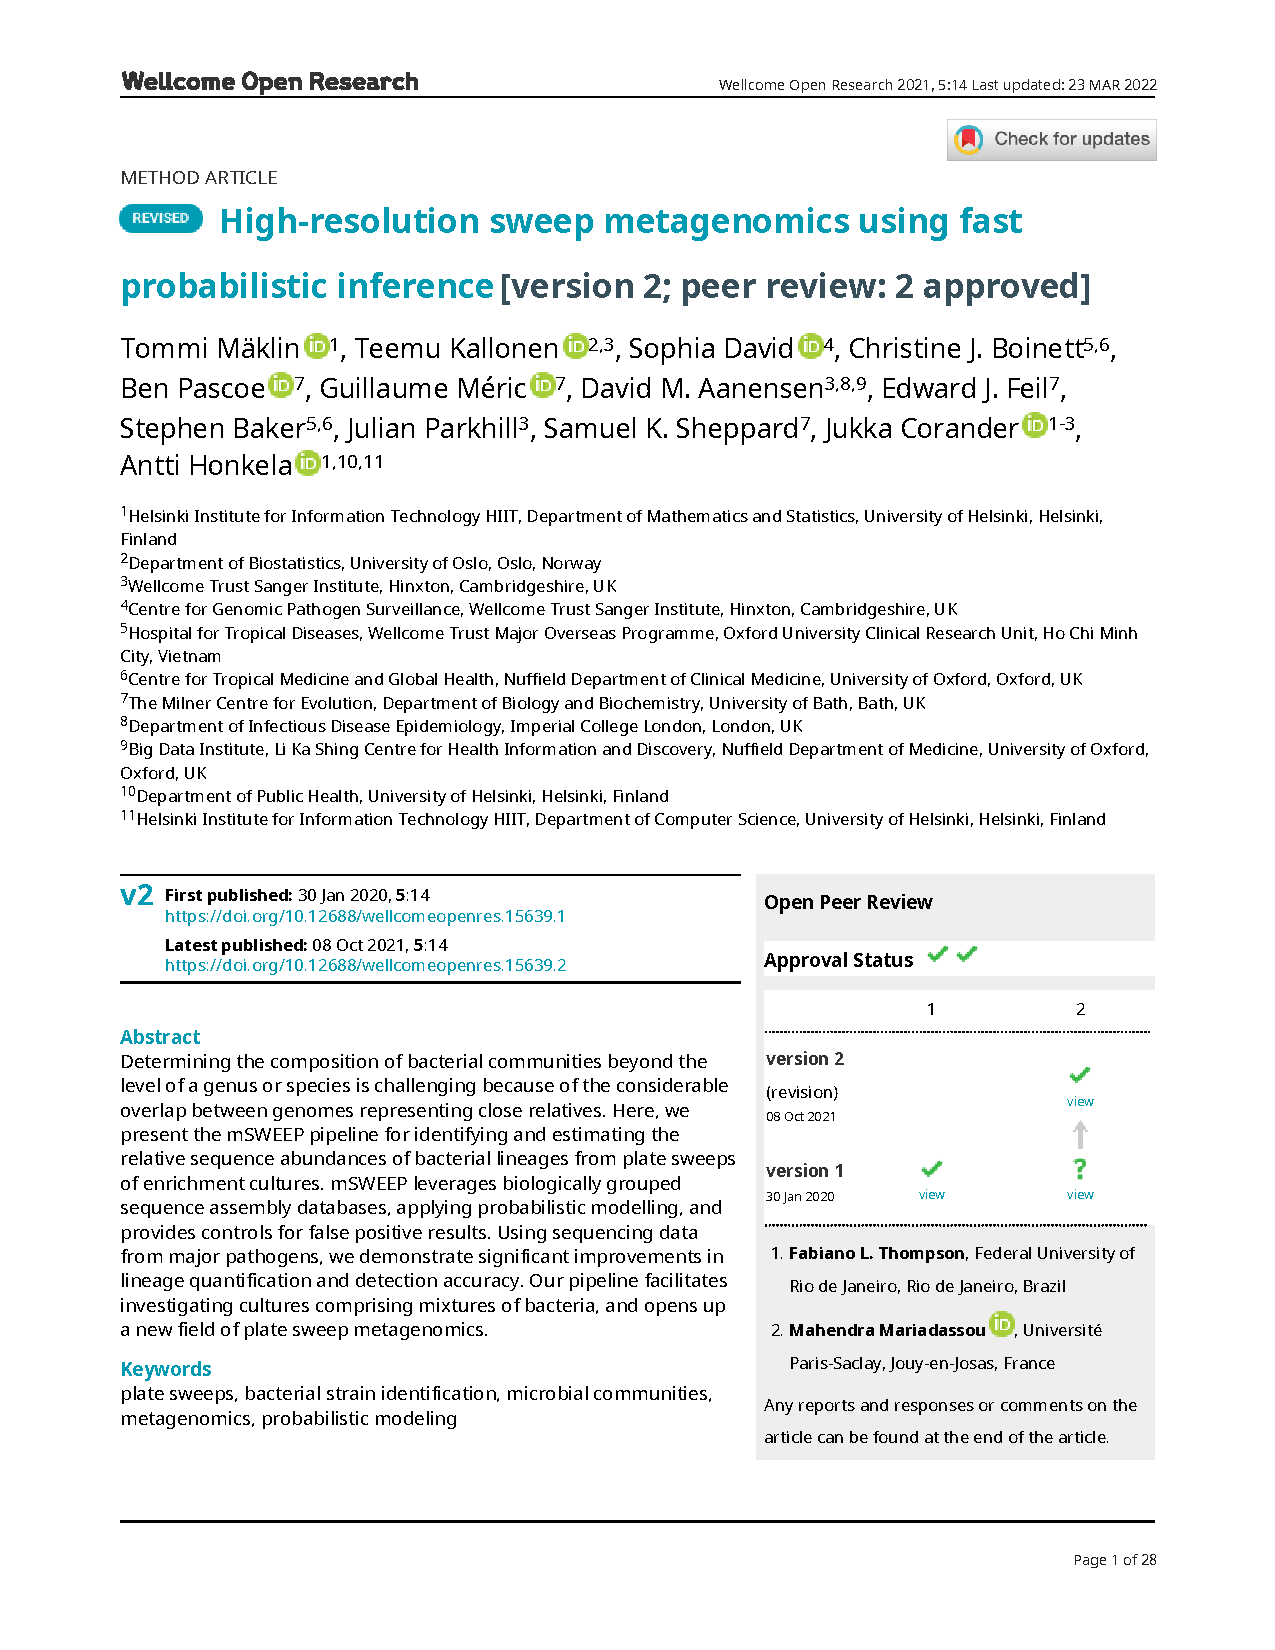
\includepdf[pages=-]{papers/maklin_high-resolution_2021.pdf}


% ******************************************************************************


\chapter*{Paper II}\thispagestyle{plain}
\addcontentsline{toc}{section}{Bacterial genomic epidemiology with mixed samples}

\note{I}{-222pt}{\dvWHITE}
%\notee{-222pt}{\dvWHITE}

\note{II}{-5pt}{black}
%\notee{-126.5pt}{\dvWHITE}

\note{III}{0pt}{\dvWHITE}
%\notee{-126.5pt}{\dvWHITE}

%% \note{IV}{-5pt}{\dvWHITE}
%% %\notee{-126.5pt}{\dvWHITE}

%% \note{V}{-5pt}{\dvWHITE}
%% %\notee{-126.5pt}{\dvWHITE}

%% \note{VI}{-5pt}{\dvWHITE}
%% %\notee{-126.5pt}{\dvWHITE}

\vspace{80pt}

% Here are the names of the authors
\underline{Tommi Mäklin}, Teemu Kallonen, Jarno Alanko, Ørjan
Samuelsen, Kristin Hegstad, Veli Mäkinen, Jukka Corander, Eva Heinz,
and Antti Honkela.

\vspace{10pt}
% Title of the 2nd paper
\noindent\textbf{Bacterial genomic epidemiology with mixed samples}

\vspace{10pt}
% Bibliographical information of the paper, for example, of a conference paper
\noindent In 
\emph{Microbial Genomics}, 
\\vol. 7 issue 11, 2021.

\vspace{60pt}
% Copyright information, for example, if the publisher is Springer
\noindent Copyright \textcopyright\ The Authors. This is an
open-access article distributed under the terms of the Creative
Commons Attribution License. This article was made open access via a
Publish and Read agreement between the Microbiology Society and the
corresponding author’s institution.

\cleardoublepage
% Including the original publication
\includepdf[pages=-]{papers/maklin_bacterial_2021.pdf}

% ******************************************************************************


\chapter*{Paper III}\thispagestyle{plain}
\addcontentsline{toc}{section}{Strong pathogen competition in neonatal gut colonization}

\note{I}{-222pt}{\dvWHITE}
%\notee{-222pt}{\dvWHITE}

\note{II}{-5pt}{\dvWHITE}
%\notee{-126.5pt}{\dvWHITE}

\note{III}{0pt}{black}
%\notee{-126.5pt}{\dvWHITE}

%% \note{IV}{-5pt}{\dvWHITE}
%% %\notee{-126.5pt}{\dvWHITE}

%% \note{V}{-5pt}{\dvWHITE}
%% %\notee{-126.5pt}{\dvWHITE}

%% \note{VI}{-5pt}{\dvWHITE}
%% %\notee{-126.5pt}{\dvWHITE}

\vspace{80pt}
% Here are the names of the authors
\underline{Tommi Mäklin}, Harry Thorpe, Anna Pöntinen, Rebecca Gladstone, Alan McNally, Ørjan
Samuelsen, Pål Johnsen, Trevor Lawley, Antti Honkela, and Jukka Corander.

\vspace{10pt}
% Title of the 3rd paper
\noindent\textbf{Strong pathogen competition in neonatal gut colonization}

\vspace{10pt}
% Bibliographical information of the paper, for example, a submitted paper
\noindent Submitted, preprint available from \emph{bioRxiv}.

\vspace{60pt}
%Copyright information, when the authors have the copyright of the paper
\noindent
The copyright holder for this preprint is the author/funder, who has
granted bioRxiv a license to display the preprint in perpetuity. It is
made available under a CC-BY 4.0 International license.

\cleardoublepage
% Including the original publication
%\includepdf[pages=-]{Publication_name_3.pdf}



% ******************************************************************************


%% \chapter*{Paper IV}\thispagestyle{empty}
%% \note{I}{-222pt}{\dvWHITE}
%% %\notee{-222pt}{\dvWHITE}

%% \note{II}{-100pt}{\dvWHITE}
%% %\notee{-126.5pt}{\dvWHITE}

%% \note{III}{-5pt}{\dvWHITE}
%% %\notee{-126.5pt}{\dvWHITE}

%% \note{IV}{-5pt}{black}
%% %\notee{-126.5pt}{\dvWHITE}

%% \note{V}{-5pt}{\dvWHITE}
%% %\notee{-126.5pt}{\dvWHITE}

%% \note{VI}{-5pt}{\dvWHITE}
%% %\notee{-126.5pt}{\dvWHITE}

%% \vspace{80pt}
%% % Here are the names of the authors
%% John Doe, Jane Doe, and John Smith

%% \vspace{10pt}
%% % Title of the 4th paper
%% \noindent\textbf{This is the title of the 4th paper}

%% \vspace{10pt}
%% % Bibliographical information of the paper, for example, of a journal paper
%% \noindent
%% In \emph{Journal name}, \\Volume xx, 20ZZ, pages XX-YY.

%% \vspace{60pt}
%% % Copyright information, when the authors have the copyright
%% \noindent Copyright \textcopyright\ The Authors.

%% \cleardoublepage
%% % Including the original publication
%% \includepdf[pages=-]{Publication_name_4.pdf}

% ******************************************************************************

\restoregeometry

%\end{document}


\end{document}
